% Options for packages loaded elsewhere
\PassOptionsToPackage{unicode}{hyperref}
\PassOptionsToPackage{hyphens}{url}
%
\documentclass[
  ignorenonframetext,
]{beamer}
\usepackage{pgfpages}
\setbeamertemplate{caption}[numbered]
\setbeamertemplate{caption label separator}{: }
\setbeamercolor{caption name}{fg=normal text.fg}
\beamertemplatenavigationsymbolsempty
% Prevent slide breaks in the middle of a paragraph
\widowpenalties 1 10000
\raggedbottom
\setbeamertemplate{part page}{
  \centering
  \begin{beamercolorbox}[sep=16pt,center]{part title}
    \usebeamerfont{part title}\insertpart\par
  \end{beamercolorbox}
}
\setbeamertemplate{section page}{
  \centering
  \begin{beamercolorbox}[sep=12pt,center]{part title}
    \usebeamerfont{section title}\insertsection\par
  \end{beamercolorbox}
}
\setbeamertemplate{subsection page}{
  \centering
  \begin{beamercolorbox}[sep=8pt,center]{part title}
    \usebeamerfont{subsection title}\insertsubsection\par
  \end{beamercolorbox}
}
\AtBeginPart{
  \frame{\partpage}
}
\AtBeginSection{
  \ifbibliography
  \else
    \frame{\sectionpage}
  \fi
}
\AtBeginSubsection{
  \frame{\subsectionpage}
}

\usepackage{amsmath,amssymb}
\usepackage{iftex}
\ifPDFTeX
  \usepackage[T1]{fontenc}
  \usepackage[utf8]{inputenc}
  \usepackage{textcomp} % provide euro and other symbols
\else % if luatex or xetex
  \usepackage{unicode-math}
  \defaultfontfeatures{Scale=MatchLowercase}
  \defaultfontfeatures[\rmfamily]{Ligatures=TeX,Scale=1}
\fi
\usepackage{lmodern}
\ifPDFTeX\else  
    % xetex/luatex font selection
\fi
% Use upquote if available, for straight quotes in verbatim environments
\IfFileExists{upquote.sty}{\usepackage{upquote}}{}
\IfFileExists{microtype.sty}{% use microtype if available
  \usepackage[]{microtype}
  \UseMicrotypeSet[protrusion]{basicmath} % disable protrusion for tt fonts
}{}
\makeatletter
\@ifundefined{KOMAClassName}{% if non-KOMA class
  \IfFileExists{parskip.sty}{%
    \usepackage{parskip}
  }{% else
    \setlength{\parindent}{0pt}
    \setlength{\parskip}{6pt plus 2pt minus 1pt}}
}{% if KOMA class
  \KOMAoptions{parskip=half}}
\makeatother
\usepackage{xcolor}
\newif\ifbibliography
\setlength{\emergencystretch}{3em} % prevent overfull lines
\setcounter{secnumdepth}{-\maxdimen} % remove section numbering

\usepackage{color}
\usepackage{fancyvrb}
\newcommand{\VerbBar}{|}
\newcommand{\VERB}{\Verb[commandchars=\\\{\}]}
\DefineVerbatimEnvironment{Highlighting}{Verbatim}{commandchars=\\\{\}}
% Add ',fontsize=\small' for more characters per line
\usepackage{framed}
\definecolor{shadecolor}{RGB}{241,243,245}
\newenvironment{Shaded}{\begin{snugshade}}{\end{snugshade}}
\newcommand{\AlertTok}[1]{\textcolor[rgb]{0.68,0.00,0.00}{#1}}
\newcommand{\AnnotationTok}[1]{\textcolor[rgb]{0.37,0.37,0.37}{#1}}
\newcommand{\AttributeTok}[1]{\textcolor[rgb]{0.40,0.45,0.13}{#1}}
\newcommand{\BaseNTok}[1]{\textcolor[rgb]{0.68,0.00,0.00}{#1}}
\newcommand{\BuiltInTok}[1]{\textcolor[rgb]{0.00,0.23,0.31}{#1}}
\newcommand{\CharTok}[1]{\textcolor[rgb]{0.13,0.47,0.30}{#1}}
\newcommand{\CommentTok}[1]{\textcolor[rgb]{0.37,0.37,0.37}{#1}}
\newcommand{\CommentVarTok}[1]{\textcolor[rgb]{0.37,0.37,0.37}{\textit{#1}}}
\newcommand{\ConstantTok}[1]{\textcolor[rgb]{0.56,0.35,0.01}{#1}}
\newcommand{\ControlFlowTok}[1]{\textcolor[rgb]{0.00,0.23,0.31}{\textbf{#1}}}
\newcommand{\DataTypeTok}[1]{\textcolor[rgb]{0.68,0.00,0.00}{#1}}
\newcommand{\DecValTok}[1]{\textcolor[rgb]{0.68,0.00,0.00}{#1}}
\newcommand{\DocumentationTok}[1]{\textcolor[rgb]{0.37,0.37,0.37}{\textit{#1}}}
\newcommand{\ErrorTok}[1]{\textcolor[rgb]{0.68,0.00,0.00}{#1}}
\newcommand{\ExtensionTok}[1]{\textcolor[rgb]{0.00,0.23,0.31}{#1}}
\newcommand{\FloatTok}[1]{\textcolor[rgb]{0.68,0.00,0.00}{#1}}
\newcommand{\FunctionTok}[1]{\textcolor[rgb]{0.28,0.35,0.67}{#1}}
\newcommand{\ImportTok}[1]{\textcolor[rgb]{0.00,0.46,0.62}{#1}}
\newcommand{\InformationTok}[1]{\textcolor[rgb]{0.37,0.37,0.37}{#1}}
\newcommand{\KeywordTok}[1]{\textcolor[rgb]{0.00,0.23,0.31}{\textbf{#1}}}
\newcommand{\NormalTok}[1]{\textcolor[rgb]{0.00,0.23,0.31}{#1}}
\newcommand{\OperatorTok}[1]{\textcolor[rgb]{0.37,0.37,0.37}{#1}}
\newcommand{\OtherTok}[1]{\textcolor[rgb]{0.00,0.23,0.31}{#1}}
\newcommand{\PreprocessorTok}[1]{\textcolor[rgb]{0.68,0.00,0.00}{#1}}
\newcommand{\RegionMarkerTok}[1]{\textcolor[rgb]{0.00,0.23,0.31}{#1}}
\newcommand{\SpecialCharTok}[1]{\textcolor[rgb]{0.37,0.37,0.37}{#1}}
\newcommand{\SpecialStringTok}[1]{\textcolor[rgb]{0.13,0.47,0.30}{#1}}
\newcommand{\StringTok}[1]{\textcolor[rgb]{0.13,0.47,0.30}{#1}}
\newcommand{\VariableTok}[1]{\textcolor[rgb]{0.07,0.07,0.07}{#1}}
\newcommand{\VerbatimStringTok}[1]{\textcolor[rgb]{0.13,0.47,0.30}{#1}}
\newcommand{\WarningTok}[1]{\textcolor[rgb]{0.37,0.37,0.37}{\textit{#1}}}

\providecommand{\tightlist}{%
  \setlength{\itemsep}{0pt}\setlength{\parskip}{0pt}}\usepackage{longtable,booktabs,array}
\usepackage{calc} % for calculating minipage widths
\usepackage{caption}
% Make caption package work with longtable
\makeatletter
\def\fnum@table{\tablename~\thetable}
\makeatother
\usepackage{graphicx}
\makeatletter
\def\maxwidth{\ifdim\Gin@nat@width>\linewidth\linewidth\else\Gin@nat@width\fi}
\def\maxheight{\ifdim\Gin@nat@height>\textheight\textheight\else\Gin@nat@height\fi}
\makeatother
% Scale images if necessary, so that they will not overflow the page
% margins by default, and it is still possible to overwrite the defaults
% using explicit options in \includegraphics[width, height, ...]{}
\setkeys{Gin}{width=\maxwidth,height=\maxheight,keepaspectratio}
% Set default figure placement to htbp
\makeatletter
\def\fps@figure{htbp}
\makeatother

\usepackage{booktabs}
\usepackage{caption}
\usepackage{longtable}
\usepackage{colortbl}
\usepackage{array}
\usepackage{anyfontsize}
\usepackage{multirow}
\makeatletter
\@ifpackageloaded{caption}{}{\usepackage{caption}}
\AtBeginDocument{%
\ifdefined\contentsname
  \renewcommand*\contentsname{Table of contents}
\else
  \newcommand\contentsname{Table of contents}
\fi
\ifdefined\listfigurename
  \renewcommand*\listfigurename{List of Figures}
\else
  \newcommand\listfigurename{List of Figures}
\fi
\ifdefined\listtablename
  \renewcommand*\listtablename{List of Tables}
\else
  \newcommand\listtablename{List of Tables}
\fi
\ifdefined\figurename
  \renewcommand*\figurename{Figure}
\else
  \newcommand\figurename{Figure}
\fi
\ifdefined\tablename
  \renewcommand*\tablename{Table}
\else
  \newcommand\tablename{Table}
\fi
}
\@ifpackageloaded{float}{}{\usepackage{float}}
\floatstyle{ruled}
\@ifundefined{c@chapter}{\newfloat{codelisting}{h}{lop}}{\newfloat{codelisting}{h}{lop}[chapter]}
\floatname{codelisting}{Listing}
\newcommand*\listoflistings{\listof{codelisting}{List of Listings}}
\makeatother
\makeatletter
\makeatother
\makeatletter
\@ifpackageloaded{caption}{}{\usepackage{caption}}
\@ifpackageloaded{subcaption}{}{\usepackage{subcaption}}
\makeatother

\ifLuaTeX
  \usepackage{selnolig}  % disable illegal ligatures
\fi
\usepackage{bookmark}

\IfFileExists{xurl.sty}{\usepackage{xurl}}{} % add URL line breaks if available
\urlstyle{same} % disable monospaced font for URLs
\hypersetup{
  pdftitle={Gaussian Copulas for Large Spatial Fields},
  pdfauthor={Brynjólfur Gauti Guðrúnar Jónsson},
  hidelinks,
  pdfcreator={LaTeX via pandoc}}


\title{Gaussian Copulas for Large Spatial Fields}
\subtitle{Modeling Data-Level Spatial Dependence in Multivariate
Generalized Extreme Value Distributions}
\author{Brynjólfur Gauti Guðrúnar Jónsson}
\date{}
\institute{University of Iceland}

\begin{document}
\frame{\titlepage}


\begin{frame}{Introduction}
\phantomsection\label{introduction}
\begin{columns}[T]
\begin{column}{0.7\textwidth}
\begin{itemize}
\tightlist
\item
  UKCP Local Projections on a 5km grid over the UK (1980-2080)
\item
  Challenge: Modeling maximum daily precipitation in yearly blocks

  \begin{itemize}
  \tightlist
  \item
    43,920 spatial locations on a 180 x 244 grid
  \end{itemize}
\item
  Two aspects of spatial dependence:

  \begin{enumerate}
  \tightlist
  \item
    GEV parameters (ICAR models)
  \item
    Data-level dependence (Copulas)
  \end{enumerate}
\end{itemize}
\end{column}

\begin{column}{0.3\textwidth}
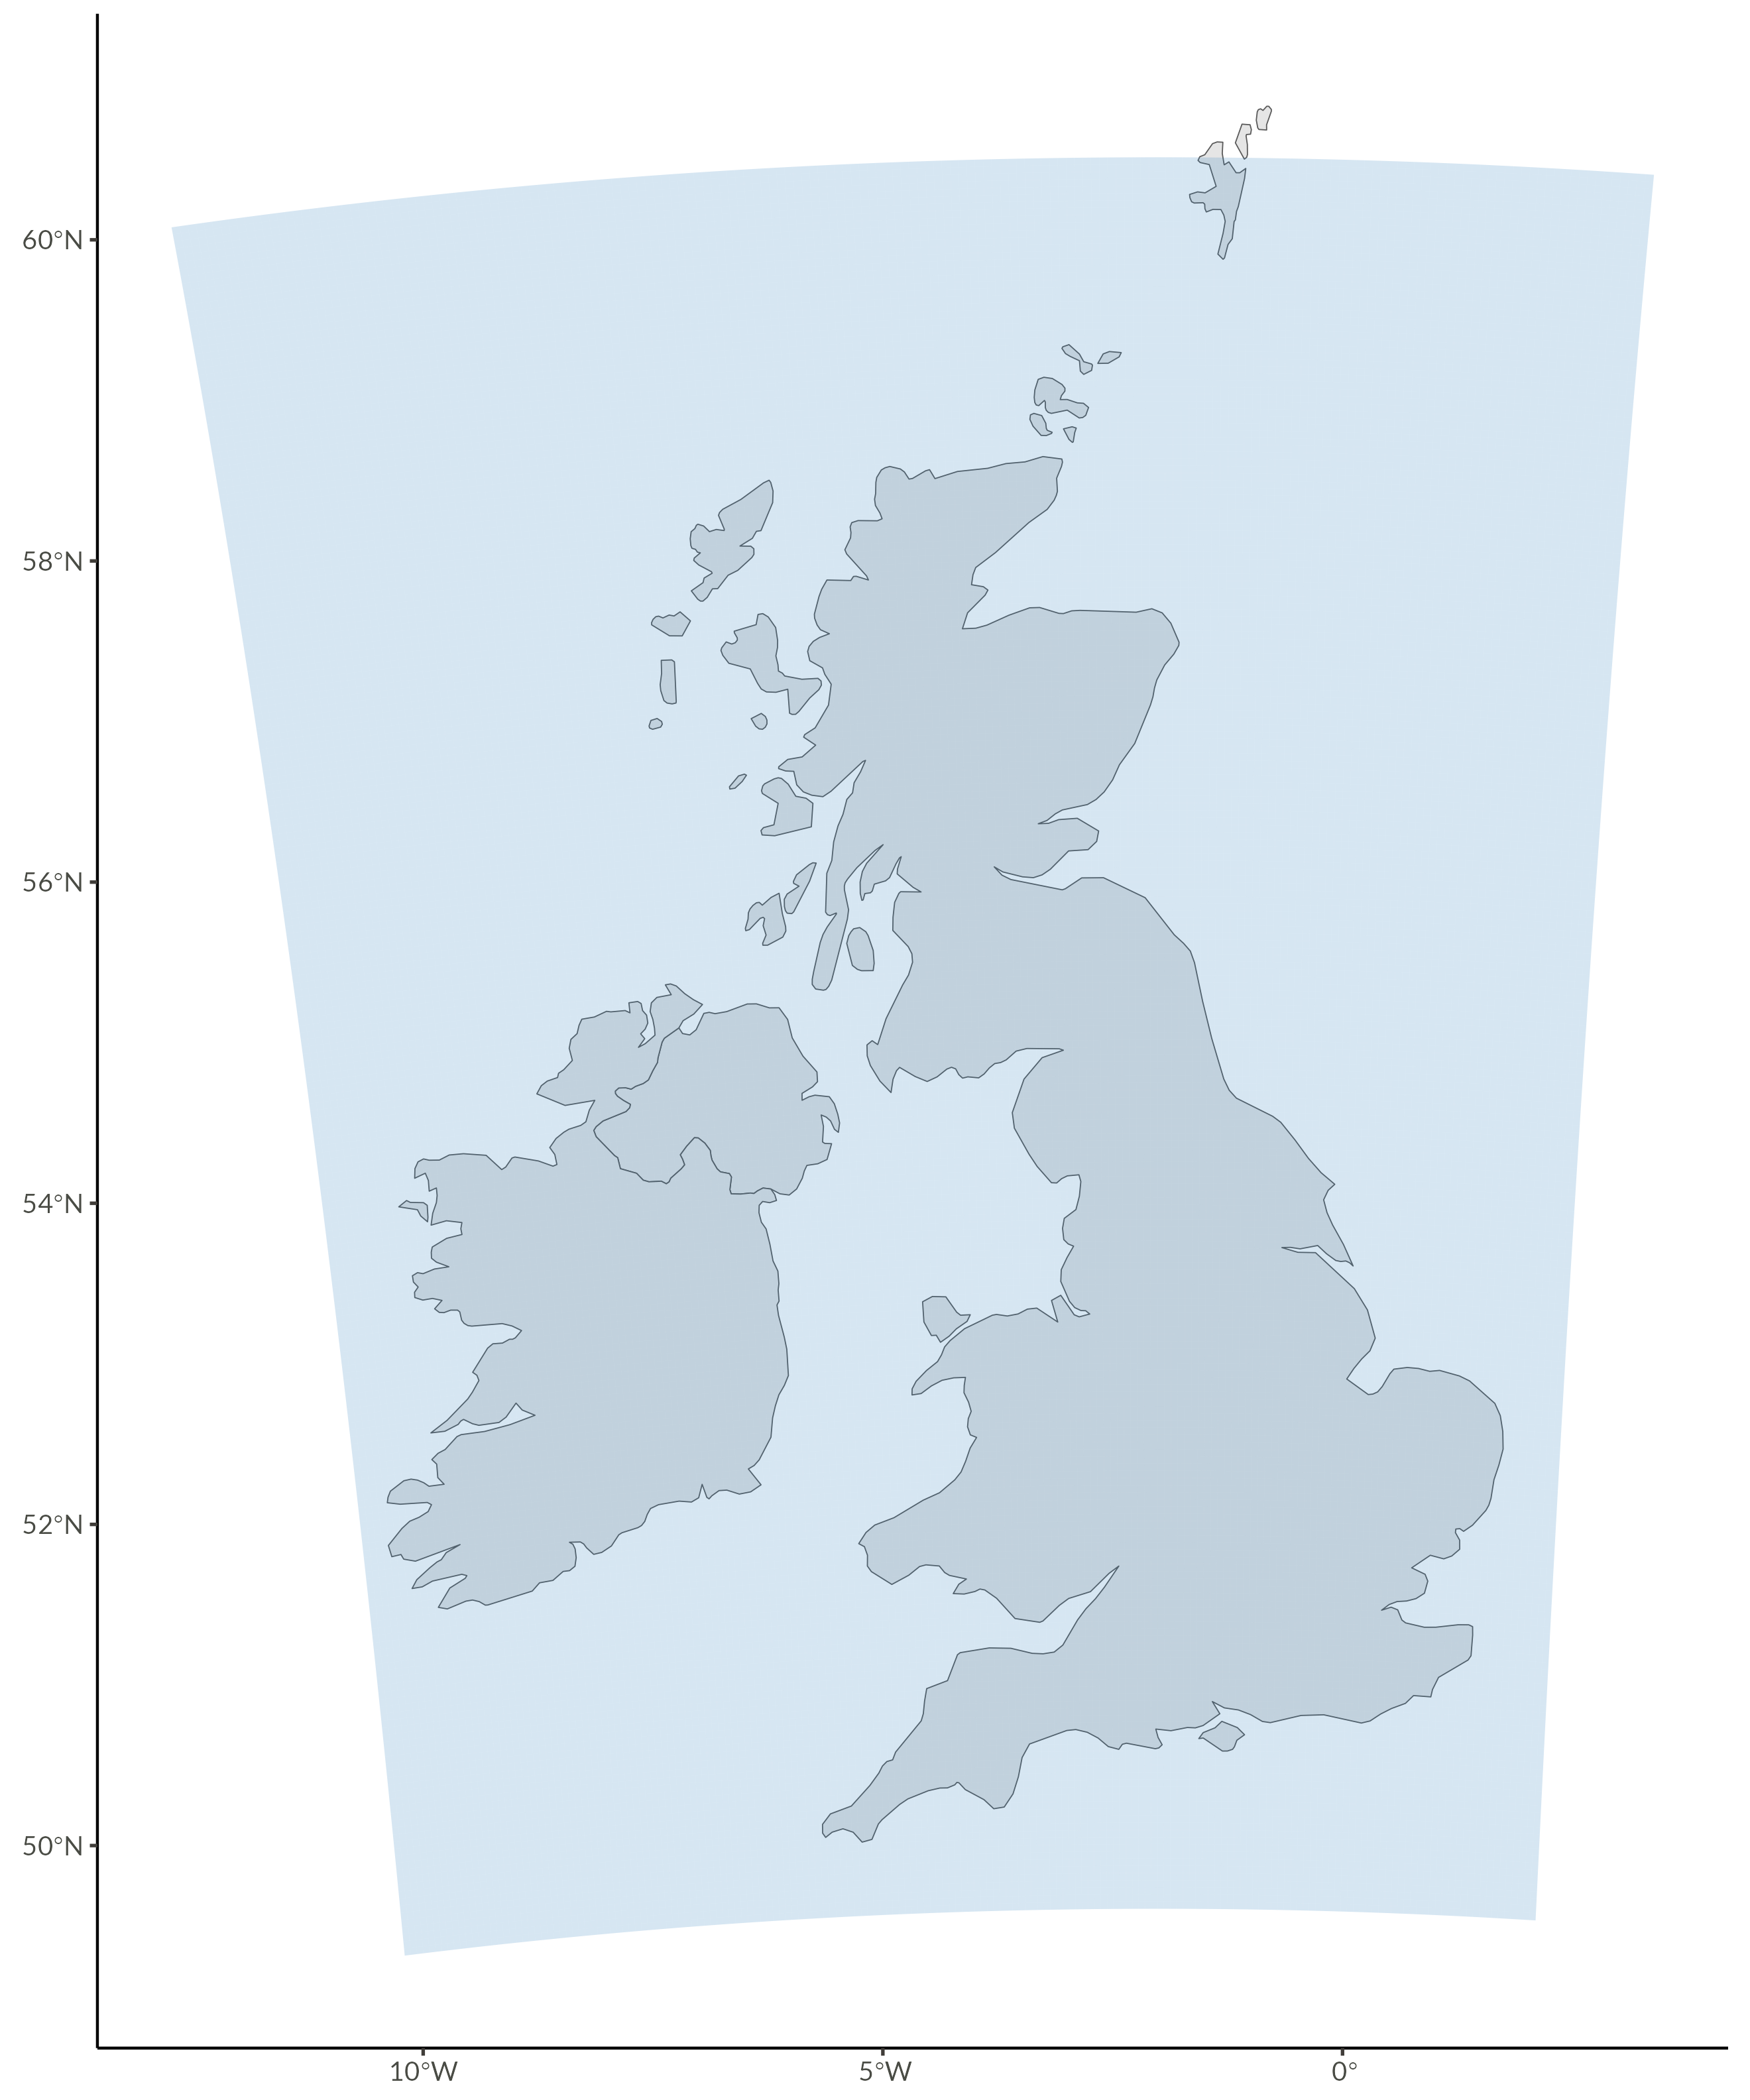
\includegraphics[width=1\textwidth,height=\textheight]{images/ukcp_data.png}
\end{column}
\end{columns}
\end{frame}

\begin{frame}{Calculating Multivariate Normal Densities}
\phantomsection\label{calculating-multivariate-normal-densities}
\begin{columns}[T]
\begin{column}{0.5\textwidth}
\begin{block}{Log Density Formula}
\phantomsection\label{log-density-formula}
\[
\log f(\mathbf{x}) \propto \frac{1}{2}\left(\log |\mathbf{Q}| - \mathbf{x}^T\mathbf{Q}\mathbf{x}\right)
\]
\end{block}

\begin{block}{Key Components}
\phantomsection\label{key-components}
\begin{enumerate}
\tightlist
\item
  \textbf{Log Determinant}: \(\log |\mathbf{Q}|\)

  \begin{itemize}
  \tightlist
  \item
    Constant for a given precision matrix
  \end{itemize}
\item
  \textbf{Quadratic Form}: \(\mathbf{x}^T\mathbf{Q}\mathbf{x}\)

  \begin{itemize}
  \tightlist
  \item
    Needs calculation for each density evaluation
  \end{itemize}
\end{enumerate}
\end{block}
\end{column}

\begin{column}{0.5\textwidth}
\begin{block}{Computational Challenges}
\phantomsection\label{computational-challenges}
\begin{itemize}
\tightlist
\item
  Log determinant calculation

  \begin{itemize}
  \tightlist
  \item
    Time complexity: \(O(n^3)\) for naive methods
  \item
    Memory complexity: \(O(n^2)\)
  \end{itemize}
\item
  Quadratic form calculation

  \begin{itemize}
  \tightlist
  \item
    Time complexity: \(O(n^2)\)
  \item
    Critical for performance in large spatial fields
  \end{itemize}
\end{itemize}
\end{block}

\begin{block}{Spatial Model Considerations}
\phantomsection\label{spatial-model-considerations}
\begin{itemize}
\tightlist
\item
  Some models (e.g., ICAR) avoid log determinant calculation
\item
  Efficient computation crucial for large-scale applications
\end{itemize}
\end{block}
\end{column}
\end{columns}
\end{frame}

\begin{frame}{Spatial Models}
\phantomsection\label{spatial-models}
\begin{columns}[T]
\begin{block}{Conditional Autoregression (CAR)}
\phantomsection\label{conditional-autoregression-car}
\begin{column}{0.5\textwidth}
\begin{itemize}
\tightlist
\item
  \(\mathbf{D}\) is a diagonal matrix with \(D_{ii} = n_i\), the number
  of neighbours of \(i\)
\item
  \(\mathbf{A}\) is the adjacency matrix with \(A_{ij} = A_{ji} = 1\) if
  \(i \sim j\)
\item
  \(\tau\) models overall precision
\end{itemize}
\end{column}

\begin{column}{0.5\textwidth}
\[
\begin{aligned}
\mathbf{x} &\sim N(\mathbf{0}, \tau \mathbf{Q}) \\
\mathbf{Q} &= \mathbf{D}\left(\mathbf{I} - \alpha \mathbf{A} \right)
\end{aligned}
\]
\end{column}
\end{block}
\end{columns}

\begin{center}\rule{0.5\linewidth}{0.5pt}\end{center}

\begin{columns}[T]
\begin{block}{Besag's Intrinsic Conditional Autoregression (ICAR)}
\phantomsection\label{besags-intrinsic-conditional-autoregression-icar}
\begin{column}{0.5\textwidth}
\begin{itemize}
\tightlist
\item
  \(\alpha = 1\), so \(\mathbf Q\) is singular, but constant
\item
  Don't have to calculate \(\log |\mathbf{Q}|\)
\item
  \(\tau\) is a precision parameter
\end{itemize}
\end{column}

\begin{column}{0.5\textwidth}
\[
\begin{aligned}
\mathbf{x} &\sim N(\mathbf{0}, \tau \mathbf{Q}) \\
\mathbf{Q} &= \mathbf{D} - \mathbf{W}
\end{aligned}
\]
\end{column}
\end{block}
\end{columns}

\begin{center}\rule{0.5\linewidth}{0.5pt}\end{center}

\begin{columns}[T]
\begin{block}{BYM (Besag-York-Mollié) Model}
\phantomsection\label{bym-besag-york-molliuxe9-model}
\begin{column}{0.5\textwidth}
\begin{itemize}
\tightlist
\item
  \(\mathbf{u}\) is the structured spatial component (Besag model)
\item
  \(\mathbf{v}\) is the unstructured component (i.i.d. normal)
\item
  \(\tau_u\) and \(\tau_v\) are precision parameters for each component
\end{itemize}
\end{column}

\begin{column}{0.5\textwidth}
\[
\begin{aligned}
\mathbf{x} &= \mathbf{u} + \mathbf{v} \\
\mathbf{u} &\sim \mathrm{ICAR}(\tau_u) \\
\mathbf{v} &\sim N(\mathbf{0}, \tau_v^{-1})
\end{aligned}
\]
\end{column}
\end{block}
\end{columns}

\begin{center}\rule{0.5\linewidth}{0.5pt}\end{center}

\begin{columns}[T]
\begin{block}{BYM2 Model}
\phantomsection\label{bym2-model}
\begin{column}{0.5\textwidth}
\begin{itemize}
\tightlist
\item
  Rewrite the combination to get proper scaling
\item
  \(\rho\) models how much of variance is spatial
\item
  \(s\) is a scaling factor chosen to make
  \(\mathrm{Var}(\mathbf u_i) \approx 1\)
\end{itemize}
\end{column}

\begin{column}{0.5\textwidth}
\[
\begin{aligned}
\mathbf{x} &= \left(\left(\sqrt{\rho/s}\right)\mathbf{u} + \left(\sqrt{1 - \rho}\right) \mathbf{v} \right)\sigma \\
\mathbf{u} &\sim \mathrm{ICAR}(1) \\
\mathbf{v} &\sim N(\mathbf{0}, n)
\end{aligned}
\]
\end{column}
\end{block}
\end{columns}
\end{frame}

\begin{frame}{Spatial Modeling on Parameter-level}
\phantomsection\label{spatial-modeling-on-parameter-level}
\begin{columns}[T]
\begin{column}{0.5\textwidth}
\begin{itemize}
\tightlist
\item
  \(\mu\): location parameter

  \begin{itemize}
  \tightlist
  \item
    \(\mu = \mu_0 \left(1 + \Delta \left(t - t_0\right)\right)\)
  \item
    Model \(\mu_0\) and trend \(\Delta\)
  \end{itemize}
\item
  \(\sigma\): scale parameter
\item
  \(\xi\): shape parameter \[
  \begin{aligned}
  \log(\mu_0) = \psi &\sim \mathrm{BYM2}(\mu_\psi, \rho_\psi, \sigma_\psi) \\
  \log(\mu_0) - \log(\sigma) = \tau &\sim \mathrm{BYM2}(\mu_\tau, \rho_\tau, \sigma_\tau) \\
  f_\xi(\xi) = \phi &\sim \mathrm{BYM2}(\mu_\phi, \rho_\phi, \sigma_\phi) \\
  f_\Delta(\Delta) = \gamma &\sim \mathrm{BYM2}(\mu_\gamma, \rho_\gamma, \sigma_\gamma)
  \end{aligned}
  \] 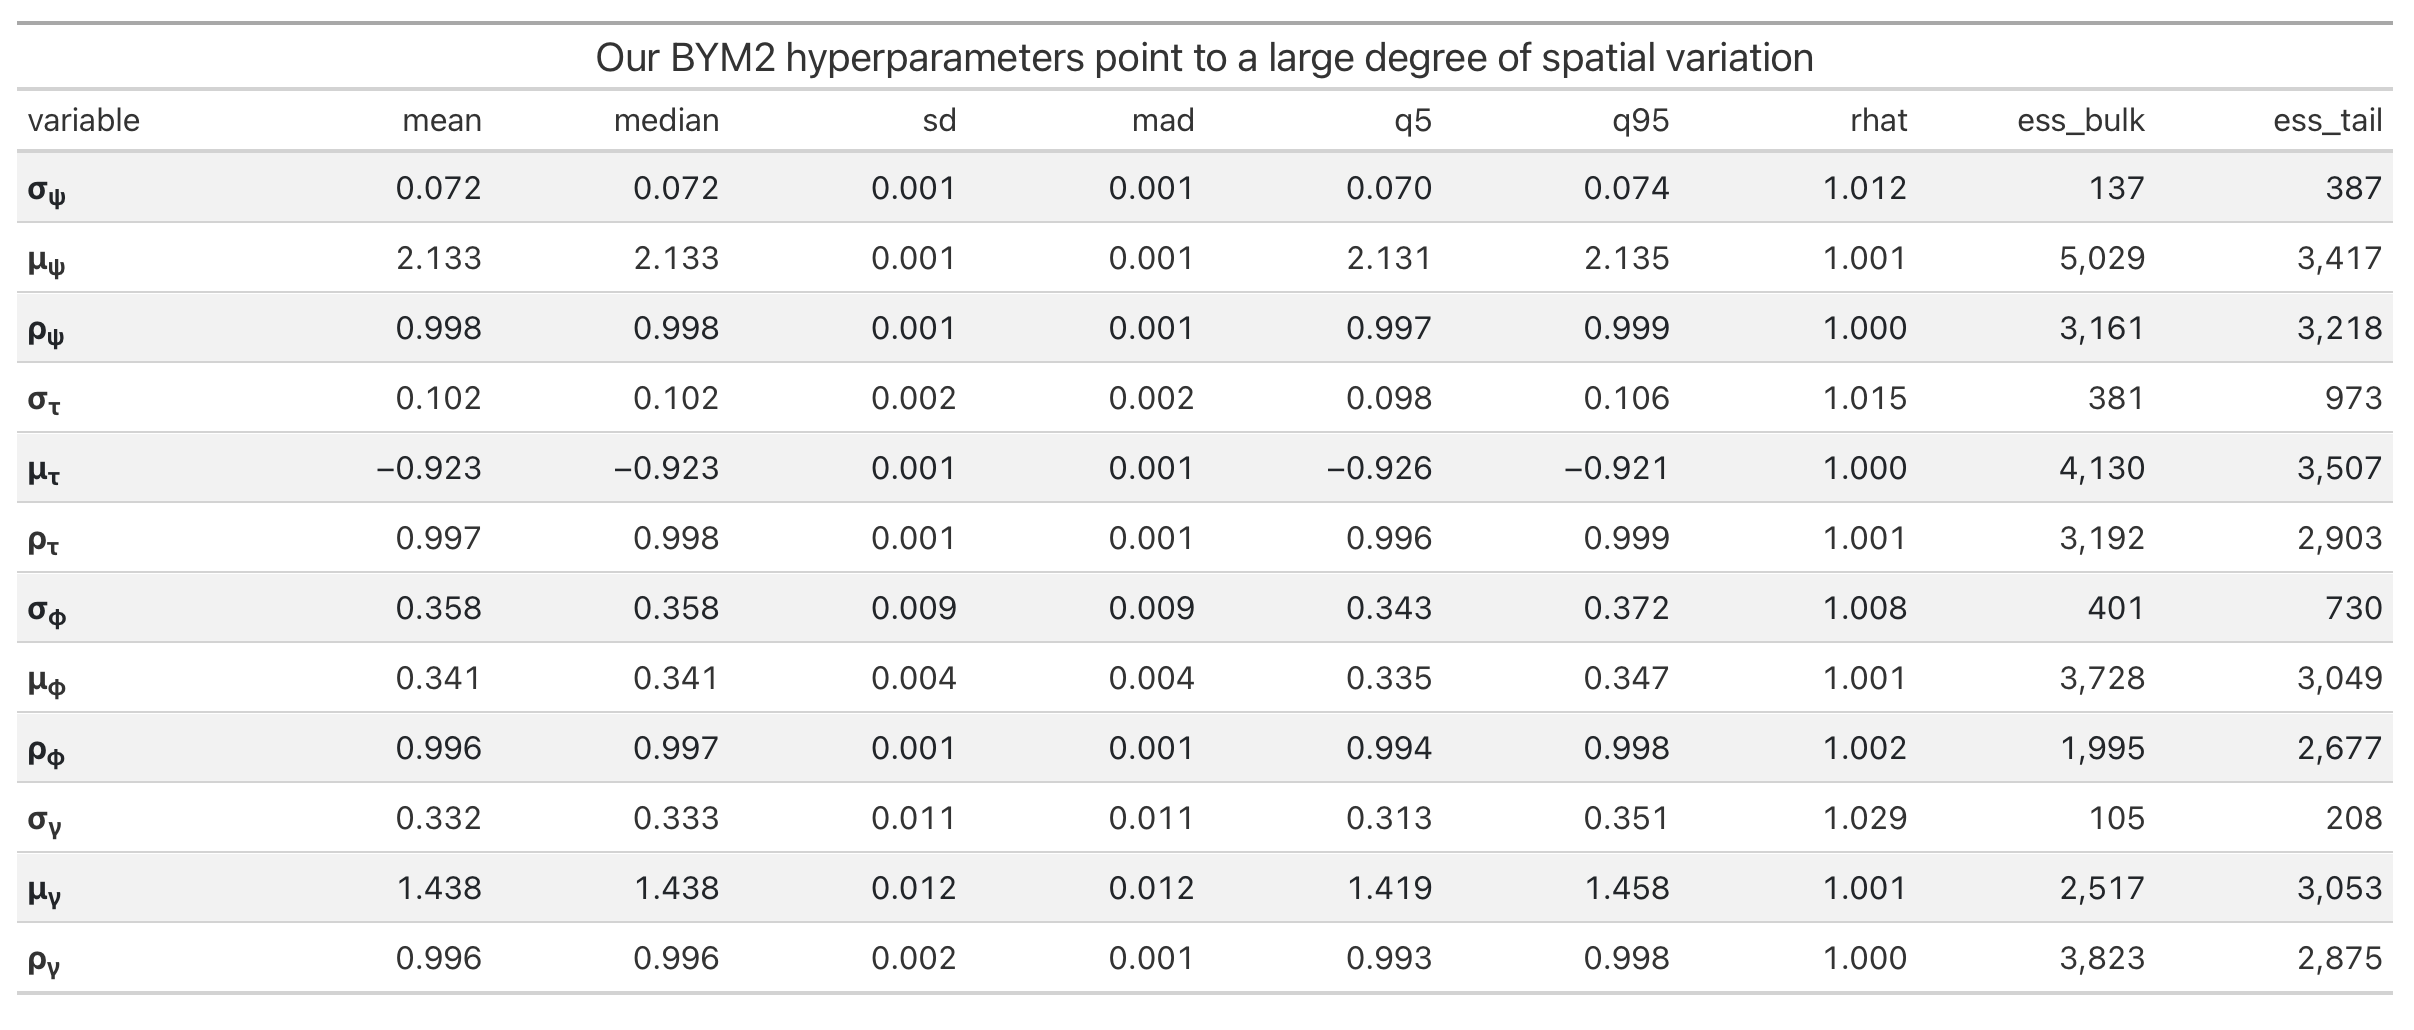
\includegraphics{images/bym_table.png}
\end{itemize}
\end{column}

\begin{column}{0.5\textwidth}
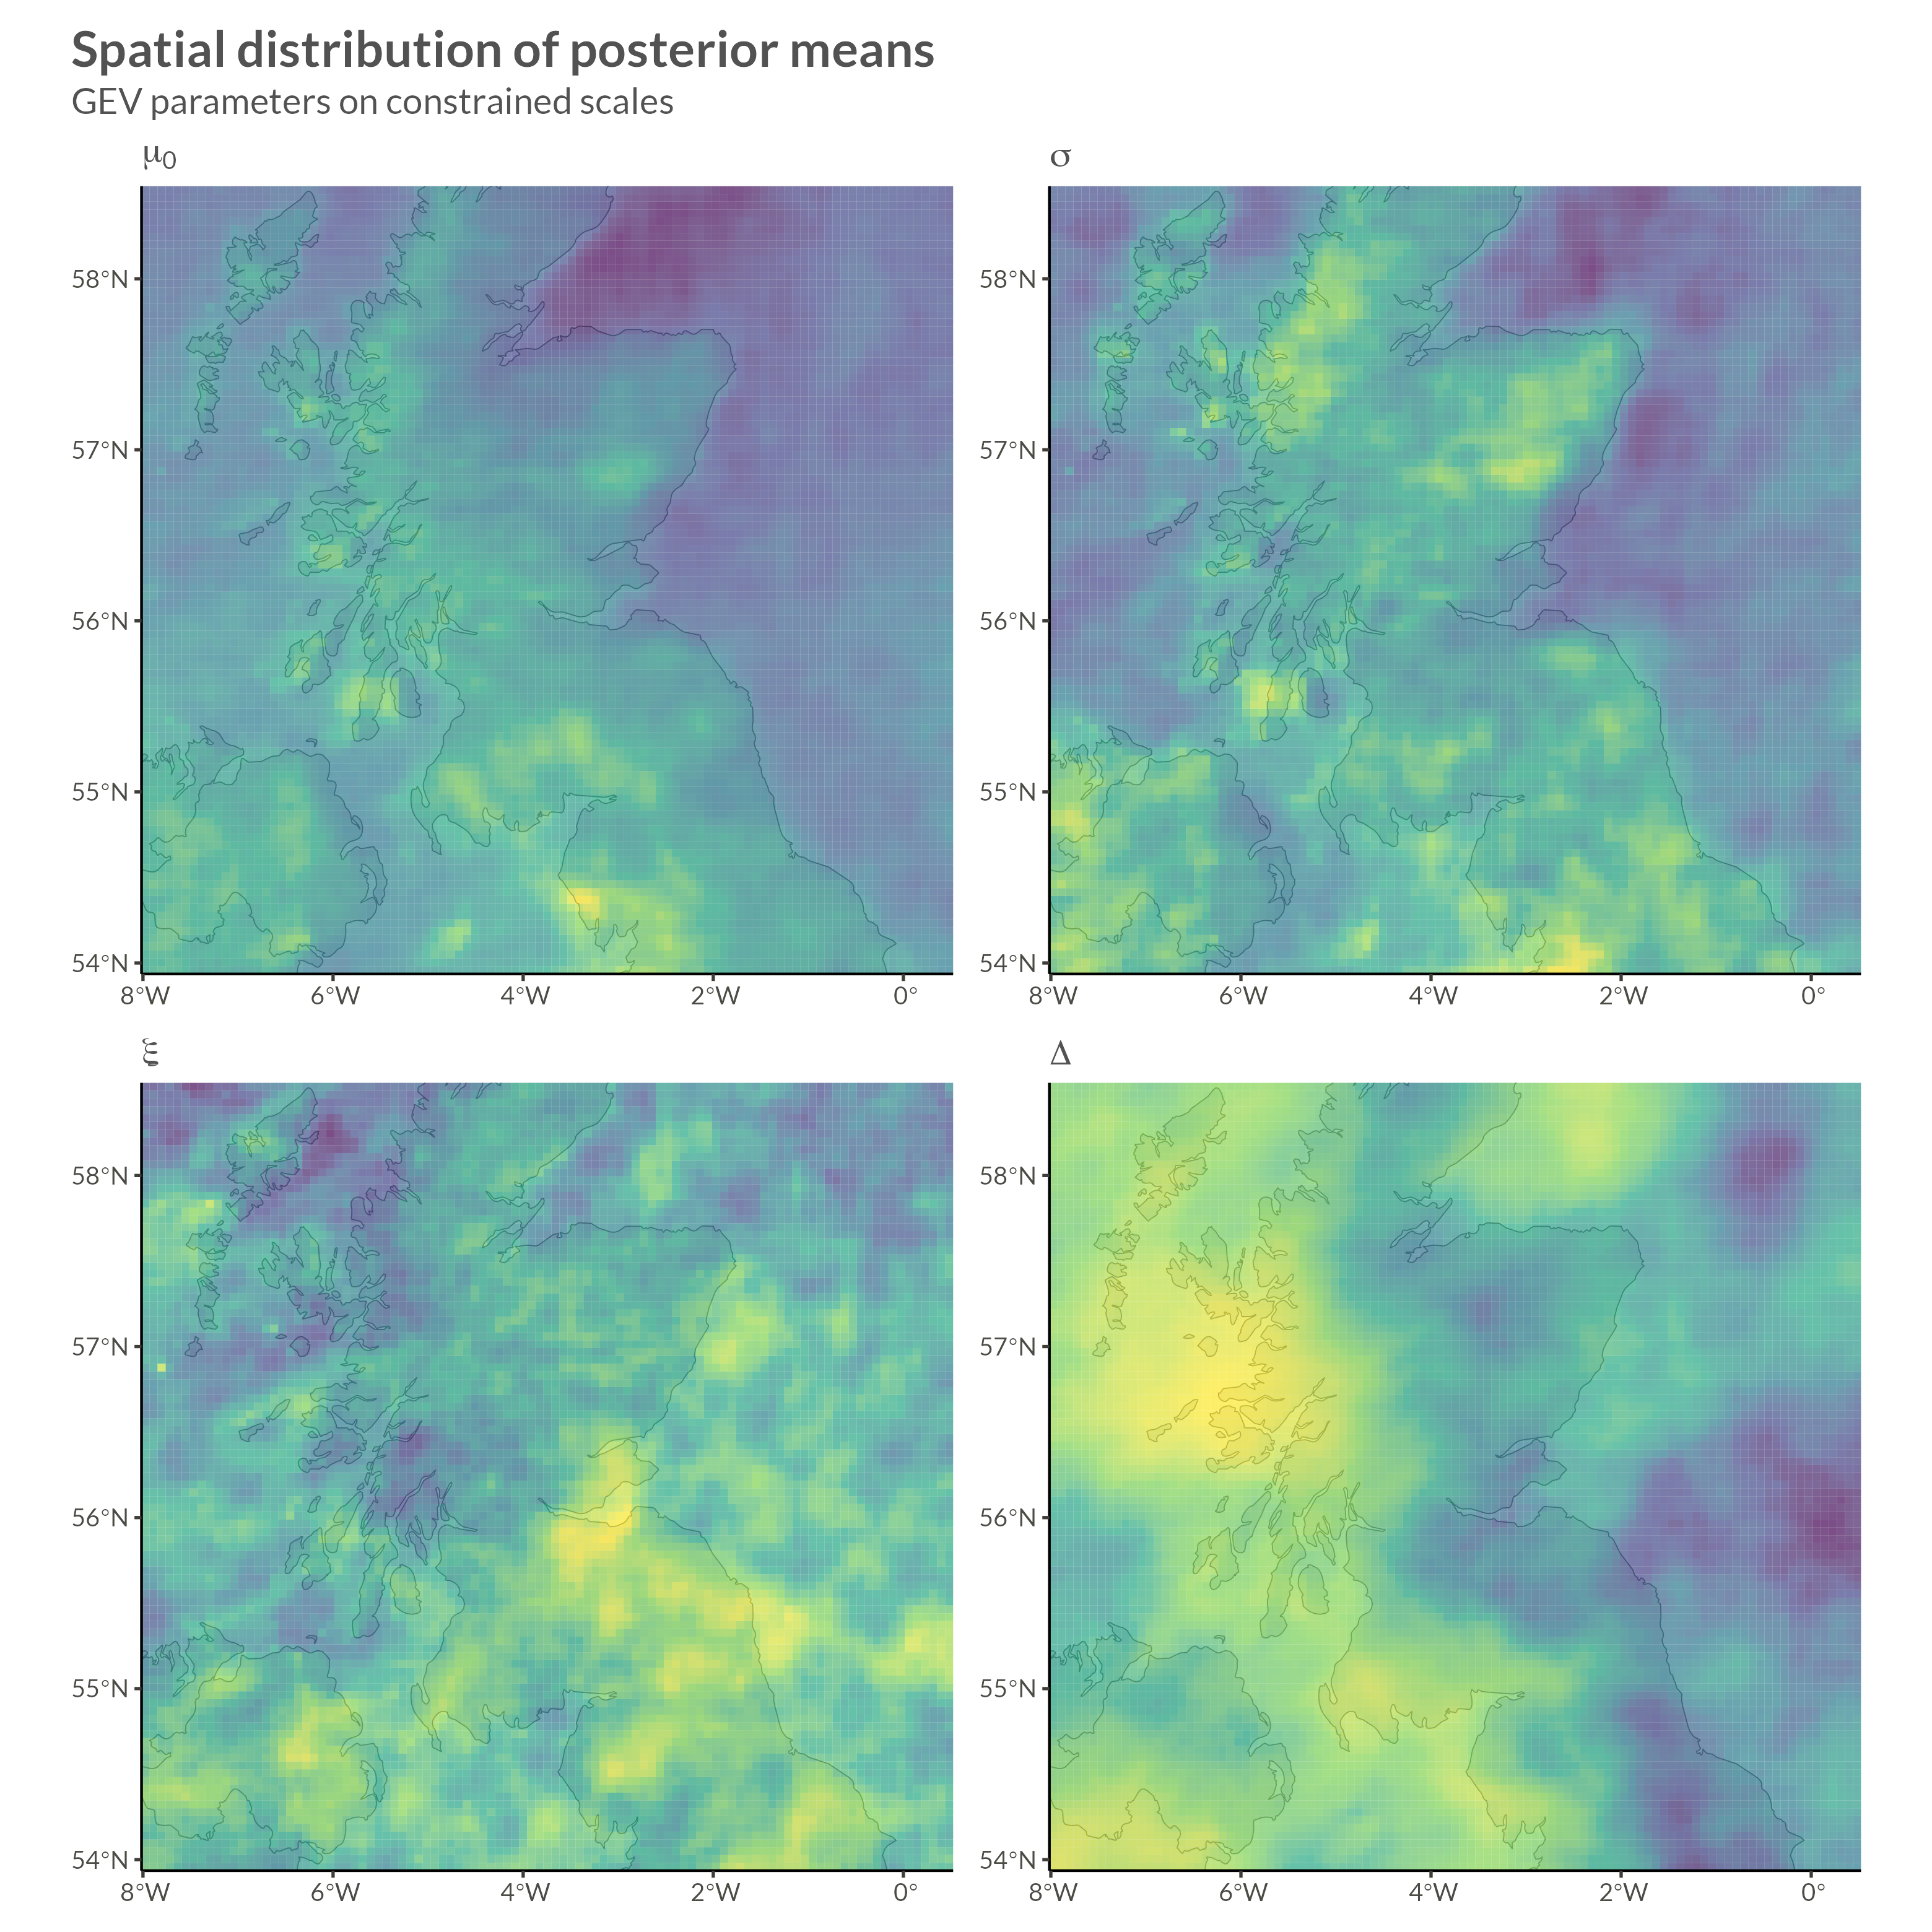
\includegraphics{images/facet_constrained.png}
\end{column}
\end{columns}
\end{frame}

\begin{frame}{From Parameter-level to Data-level Dependence}
\phantomsection\label{from-parameter-level-to-data-level-dependence}
\begin{columns}[T]
\begin{column}{0.5\textwidth}
\begin{block}{Parameter-level Dependence}
\phantomsection\label{parameter-level-dependence}
\begin{itemize}
\tightlist
\item
  Assumes conditional independence
\item
  Biased joint probability estimates
\item
  Underestimates parameter variance
\end{itemize}
\end{block}
\end{column}

\begin{column}{0.5\textwidth}
\begin{block}{Copula}
\phantomsection\label{copula}
\begin{itemize}
\tightlist
\item
  Improves joint probabilities
\item
  Enhances spatial risk assessment
\item
  Better variance estimates
\end{itemize}
\end{block}
\end{column}
\end{columns}

\textbf{Sklar's Theorem}: For any multivariate distribution \(H\), there
exists a unique copula \(C\) such that:

\[
H(\mathbf x) = C(F_1(x_1), \dots, F_d(x_d))
\]

where \(F_i\) are marginal distributions. We can also write this as a
density

\[
h(x) = c(F_1(x_1), \dots, F_d(x_d)) \prod_{i=1}^d f_i(x_i)
\]
\end{frame}

\begin{frame}{Our Approach: Matérn-like Gaussian Copula}
\phantomsection\label{our-approach-matuxe9rn-like-gaussian-copula}
\[
\begin{gathered}
\log h(\mathbf x) = \log c\left(F_1(x_1), \dots, F_d(x_d)\right) + \sum_{i=1}^d \log f_i(x_i)
\end{gathered}
\]

\begin{center}\rule{0.5\linewidth}{0.5pt}\end{center}

\begin{columns}[T]
\begin{block}{Marginal CDFs}
\phantomsection\label{marginal-cdfs}
\begin{column}{0.5\textwidth}
\begin{itemize}
\tightlist
\item
  \(F_i(x_i)\) is \(\mathrm{GEV}(\mu_i, \sigma_i, \xi_i)\)
\item
  Can model parameter dependence with BYM2
\end{itemize}
\end{column}

\begin{column}{0.5\textwidth}
\[
\begin{aligned}
\log h(\mathbf x) &= \log c(u_1, \dots, u_d) + \sum_{i=1}^d f_{\mathrm{GEV}}(x_i \vert \mu_i, \sigma_i, \xi_i) \\
u_i &= F_{\mathrm{GEV}}(x_i \vert \mu_i, \sigma_i, \xi_i)
\end{aligned}
\]
\end{column}
\end{block}
\end{columns}

\begin{center}\rule{0.5\linewidth}{0.5pt}\end{center}

\begin{columns}[T]
\begin{block}{Gaussian Copula}
\phantomsection\label{gaussian-copula}
\begin{column}{0.5\textwidth}
\begin{itemize}
\tightlist
\item
  Matérn-like precision matrix \(\mathbf{Q}\)
\item
  Scaled so \(\boldsymbol{\Sigma} = \mathbf{Q}^{-1}\) is correlation
  matrix
\item
  If \(\mathbf{Q} = \mathbf{I}\) simplifies to independent margins
\item
  How to generate, scale and compute with \(\mathbf{Q}\) quickly (for
  MCMC)?
\end{itemize}
\end{column}

\begin{column}{0.5\textwidth}
\[
\begin{aligned}
\log c(\mathbf u) &\propto \frac{1}{2}\left(\log |\mathbf{Q}| - \mathbf{z}^T\mathbf{Q}\mathbf{z} + \mathbf{z}^T\mathbf{z}\right) \\
\mathbf{z} &= \Phi^{-1}(\mathbf u)
\end{aligned}
\]
\end{column}
\end{block}
\end{columns}
\end{frame}

\begin{frame}{The Precision Matrix}
\phantomsection\label{the-precision-matrix}
\(\mathbf Q\) defined as Kronecker sum of two AR(1) precision matrices

\[
\mathbf{Q} = \left( \mathbf{Q}_{\rho_1} \otimes \mathbf{I_{n_2}} + \mathbf{I_{n_1}} \otimes \mathbf{Q}_{\rho_2} \right)^{\nu + 1}, \quad \nu \in \{0, 1, 2\}
\]

\begin{columns}[T]
\begin{column}{0.5\textwidth}
\[
\mathbf{Q}_{\rho_{1}} = \frac{1}{1-\rho_{1}^2}
\begin{bmatrix}
1 & -\rho_{1} & 0 & \cdots & 0 \\
-\rho_{1} & 1+\rho_{1}^2 & -\rho_{1} & \cdots & 0 \\
0 & -\rho_{1} & 1+\rho_{1}^2 & \cdots & 0 \\
\vdots & \vdots & \vdots & \ddots & \vdots \\
0 & 0 & 0 & \cdots & 1
\end{bmatrix}
\]
\end{column}

\begin{column}{0.5\textwidth}
\[
\mathbf{Q}_{\rho_{2}} = \frac{1}{1-\rho_{2}^2}
\begin{bmatrix}
1 & -\rho_{2} & 0 & \cdots & 0 \\
-\rho_{2} & 1+\rho_{2}^2 & -\rho_{2} & \cdots & 0 \\
0 & -\rho_{2} & 1+\rho_{2}^2 & \cdots & 0 \\
\vdots & \vdots & \vdots & \ddots & \vdots \\
0 & 0 & 0 & \cdots & 1
\end{bmatrix}
\]
\end{column}

Which means that

\[
\mathbf Q = \begin{pmatrix}
(1+\rho_1^2)\mathbf{I_{n_2}} + \mathbf{Q_{\rho_2}} & -\rho_1\mathbf{I_{n_2}} & \dots & \cdots & \dots \\
-\rho_1\mathbf{I_{n_2}} & (1+\rho_1^2)\mathbf{I_{n_2}} + \mathbf{q_{\rho_2}} & -\rho_1 \mathbf{I_{n_2}} & \cdots & \vdots  \\
\vdots & \ddots & \ddots & \ddots & \vdots \\
\dots & \dots & \cdots & -\rho_1 \mathbf{I_{n_2}} & (1+\rho_1^2)\mathbf{I_{n_2}} + \mathbf{Q_{\rho_2}}
\end{pmatrix}^{\nu + 1}
\]
\end{columns}
\end{frame}

\begin{frame}{Eigendecomposition}
\phantomsection\label{eigendecomposition}
\begin{columns}[T]
Because of how \(\mathbf{Q}\) is defined, we know that

\[
\begin{aligned}
\mathbf{Q} &= \mathbf{V}\boldsymbol{\Lambda}\mathbf{V} \\
&= (\mathbf{V_{\rho_1}} \otimes \mathbf{V_{\rho_2}})(\boldsymbol \Lambda_{\rho_1} \otimes \mathbf{I} + \mathbf{I} \otimes \boldsymbol \Lambda_{\rho_2})^{\nu + 1}(\mathbf{V_{\rho_1}} \otimes \mathbf{V_{\rho_2}})^T
\end{aligned}
\]

where

\[
\begin{aligned}
\mathbf{Q}_{\rho_1} = \mathbf{V_{\rho_1}}\boldsymbol \Lambda_{\rho_1}\mathbf{V_{\rho_1}}^T \qquad \& \qquad
\mathbf{Q}_{\rho_2} = \mathbf{V_{\rho_2}}\boldsymbol \Lambda_{\rho_2}\mathbf{V_{\rho_2}}^T
\end{aligned}
\]

Spectral decomposition defined by value/vector pairs of smaller matrices

\begin{column}{0.5\textwidth}
\[
\left\{\lambda_{\rho_1}\right\}_i + \left\{\lambda_{\rho_2}\right\}_j
\]
\end{column}

\begin{column}{0.48\textwidth}
\[
\left\{\mathbf{v}_{\rho_1}\right\}_i \otimes \left\{\mathbf{v}_{\rho_2}\right\}_j
\]
\end{column}

\begin{itemize}
\tightlist
\item
  Problem:
  \(\boldsymbol \Sigma_{ii} = \left(\mathbf Q^{-1} \right)_{ii} \neq  1\)
\item
  Solution: \(\mathbf{\widetilde  Q} = \mathbf{D}\mathbf{Q}\mathbf{D}\),
  where \(\mathbf D_{ii} = \sqrt{\boldsymbol \Sigma_{ii}}\)
\end{itemize}
\end{columns}
\end{frame}

\begin{frame}{Marginal Standard Deviations}
\phantomsection\label{marginal-standard-deviations}
\[
\boldsymbol \Sigma = \mathbf Q^{-1} = (\mathbf{V}\boldsymbol\Lambda\mathbf{V}^T)^{-1} = \mathbf{V}\boldsymbol \Lambda^{-1}\mathbf{V}
\]

We know that if \(A = BC\) then \(A_{ii} = B_{i, .} C_{., i}\), so

\[
\boldsymbol \Sigma_{ii} = \sum_{k=1}^{n} v_{ik} \frac{1}{\lambda_k} (v^T)_{ki} = \sum_{k=1}^{n} v_{ik} \frac{1}{\lambda_k} v_{ik} = \sum_{k=1}^{n} v_{ik}^2 \frac{1}{\lambda_k}
\]

Compute vector \(\sigma^2\) containing all marginal variances

\[ 
\sigma^2 = \sum_{i = 1}^{n_1} \sum_{j=1}^{n_2} \frac{\left(\left\{\mathbf{v}_{\rho_1}\right\}_i \otimes \left\{\mathbf{v}_{\rho_2}\right\}_j\right)^{2}}{\quad\left(\left\{\lambda_{\rho_1}\right\}_i + \left\{\lambda_{\rho_2}\right\}_j\right)^{\nu+1}}
\]
\end{frame}

\begin{frame}[fragile]{Marginal Standard Deviations}
\phantomsection\label{marginal-standard-deviations-1}
\begin{columns}[T]
\begin{column}{0.58\textwidth}
\begin{Shaded}
\begin{Highlighting}[]
\NormalTok{dim1 }\OtherTok{\textless{}{-}} \DecValTok{50}\NormalTok{; dim2 }\OtherTok{\textless{}{-}} \DecValTok{50}
\NormalTok{rho1 }\OtherTok{\textless{}{-}} \FloatTok{0.5}\NormalTok{; rho2 }\OtherTok{\textless{}{-}} \FloatTok{0.3}
\NormalTok{nu }\OtherTok{\textless{}{-}} \DecValTok{2}

\NormalTok{Q1 }\OtherTok{\textless{}{-}} \FunctionTok{make\_AR\_prec\_matrix}\NormalTok{(dim1, rho1)}
\NormalTok{Q2 }\OtherTok{\textless{}{-}} \FunctionTok{make\_AR\_prec\_matrix}\NormalTok{(dim2, rho2)}

\NormalTok{I1 }\OtherTok{\textless{}{-}}\NormalTok{ Matrix}\SpecialCharTok{::}\FunctionTok{Diagonal}\NormalTok{(dim1)}
\NormalTok{I2 }\OtherTok{\textless{}{-}}\NormalTok{ Matrix}\SpecialCharTok{::}\FunctionTok{Diagonal}\NormalTok{(dim2)}

\NormalTok{Q }\OtherTok{\textless{}{-}}\NormalTok{ temp }\OtherTok{\textless{}{-}} \FunctionTok{kronecker}\NormalTok{(Q1, I2) }\SpecialCharTok{+} \FunctionTok{kronecker}\NormalTok{(I1, Q2)}
\ControlFlowTok{for}\NormalTok{ (i }\ControlFlowTok{in} \FunctionTok{seq\_len}\NormalTok{(nu)) Q }\OtherTok{\textless{}{-}}\NormalTok{ Q }\SpecialCharTok{\%*\%}\NormalTok{ temp}
\end{Highlighting}
\end{Shaded}
\end{column}

\begin{column}{0.42\textwidth}
\begin{Shaded}
\begin{Highlighting}[]
\NormalTok{msd }\OtherTok{\textless{}{-}} \ControlFlowTok{function}\NormalTok{(Q1, Q2) \{}

\NormalTok{  E1 }\OtherTok{\textless{}{-}} \FunctionTok{eigen}\NormalTok{(Q1)}
\NormalTok{  E2 }\OtherTok{\textless{}{-}} \FunctionTok{eigen}\NormalTok{(Q2)}

  \FunctionTok{marginal\_sd\_eigen}\NormalTok{(}
\NormalTok{    E1}\SpecialCharTok{$}\NormalTok{values, E1}\SpecialCharTok{$}\NormalTok{vectors, dim1,}
\NormalTok{    E2}\SpecialCharTok{$}\NormalTok{values, E2}\SpecialCharTok{$}\NormalTok{vectors, dim2,}
\NormalTok{    nu}
\NormalTok{  ) }\SpecialCharTok{|\textgreater{}} 
  \FunctionTok{sort}\NormalTok{()}
\NormalTok{\}}
\end{Highlighting}
\end{Shaded}
\end{column}
\end{columns}

\begin{Shaded}
\begin{Highlighting}[]
\NormalTok{bench}\SpecialCharTok{::}\FunctionTok{mark}\NormalTok{(}
  \StringTok{"solve"} \OtherTok{=} \FunctionTok{solve}\NormalTok{(Q) }\SpecialCharTok{|\textgreater{}} \FunctionTok{diag}\NormalTok{() }\SpecialCharTok{|\textgreater{}} \FunctionTok{sqrt}\NormalTok{() }\SpecialCharTok{|\textgreater{}} \FunctionTok{sort}\NormalTok{(),}
  \StringTok{"inla.qinv"} \OtherTok{=} \FunctionTok{inla.qinv}\NormalTok{(Q) }\SpecialCharTok{|\textgreater{}} \FunctionTok{diag}\NormalTok{() }\SpecialCharTok{|\textgreater{}} \FunctionTok{sqrt}\NormalTok{() }\SpecialCharTok{|\textgreater{}} \FunctionTok{sort}\NormalTok{(),}
  \StringTok{"marginal\_sd\_eigen"} \OtherTok{=} \FunctionTok{msd}\NormalTok{(Q1, Q2),}
  \AttributeTok{iterations =} \DecValTok{10}\NormalTok{,}
  \AttributeTok{filter\_gc =} \ConstantTok{FALSE}
\NormalTok{)}
\end{Highlighting}
\end{Shaded}

\begin{verbatim}
# A tibble: 3 x 6
  expression             min   median `itr/sec` mem_alloc `gc/sec`
  <bch:expr>        <bch:tm> <bch:tm>     <dbl> <bch:byt>    <dbl>
1 solve                1.25s    1.27s     0.777   78.17MB    0.777
2 inla.qinv         342.29ms 353.72ms     2.73     4.33MB    0    
3 marginal_sd_eigen   3.28ms   3.31ms   283.     649.35KB    0    
\end{verbatim}
\end{frame}

\begin{frame}{Calculating the (non-copula) density}
\phantomsection\label{calculating-the-non-copula-density}
The Gaussian log pdf is \[
\log f(\mathbf{u} \vert \mathbf{Q}) \propto \frac{1}{2}\left(\log|\mathbf{Q}| - \mathbf{z}^T\mathbf{Q}\mathbf{z}\right)
\]

Without scaling of \(\mathbf Q\) we get

\[
\log|\mathbf{Q}| = \sum_{k=1}^{n_1n_2}\log\lambda_k = \sum_{i=1}^{n_1}\sum_{j=2}^{n_2} \log\left[\left(\left\{\lambda_{\rho_1}\right\}_i + \left\{\lambda_{\rho_2}\right\}_j\right)^{\nu + 1}\right]
\]

\[
\mathbf{z}^T\mathbf{Q}\mathbf{z} = \sum_{k=1}^{n_1n_2}\lambda_k \left(v_k^T\mathbf z\right)^2 = 
\sum_{i=1}^{n_1}\sum_{j=2}^{n_2} 
\left(\left\{\lambda_{\rho_1}\right\}_i + \left\{\lambda_{\rho_2}\right\}_j\right)
\left[\left(\left\{\mathbf{v}_{\rho_1}\right\}_i \otimes \left\{\mathbf{v}_{\rho_2}\right\}_j\right)^T\mathbf z\right]^2
\]
\end{frame}

\begin{frame}{Calculating the copula density}
\phantomsection\label{calculating-the-copula-density}
Let
\(\mathbf v = \left\{\mathbf{v}_{\rho_1}\right\}_i \otimes \left\{\mathbf{v}_{\rho_2}\right\}_j\)
and
\(\lambda = \left(\left\{\lambda_{\rho_1}\right\}_i + \left\{\lambda_{\rho_2}\right\}_j\right)^{\nu + 1}\).
Normalise \(\mathbf v\) and \(\lambda\) with

\[
\begin{gathered}
\widetilde{\mathbf{v}} = \frac{D\mathbf{v}}{\vert\vert D\mathbf{v}\vert\vert_2}, \qquad
\widetilde{\lambda} = \vert\vert D\mathbf{v}\vert\vert_2^2 \cdot \lambda
\end{gathered}
\]

Then \(\widetilde{\mathbf{v}}\) and \(\widetilde{\lambda}\) are an
eigenvector/value pair of the scaled precision matrix
\(\mathbf{\widetilde{Q}}\). Iterate over \(i\) and \(j\) to calculate

\[
\log c(\mathbf{u} \vert \mathbf{\widetilde{Q}}) = \frac{1}{2}\log|\mathbf{\widetilde Q}| - \frac{1}{2}\mathbf{z}^T\mathbf{\widetilde Q}\mathbf{z} + \frac{1}{2}\mathbf{z}^T\mathbf{z}
\]
\end{frame}

\begin{frame}{Folded Circulant Approximation}
\phantomsection\label{folded-circulant-approximation}
\begin{columns}[T]
\begin{column}{0.4\textwidth}
\begin{block}{AR(1) precision}
\phantomsection\label{ar1-precision}
The exact form of \(Q_{\rho}\), the precision matrix of a
one-dimensional AR(1) process with correlation \(\rho\) is
\end{block}
\end{column}

\begin{column}{0.6\textwidth}
\[
\mathbf{Q}_\rho = \frac{1}{1-\rho^2}
\begin{bmatrix}
1 & -\rho & 0 & \cdots & 0 \\
-\rho & 1+\rho^2 & -\rho & \cdots & 0 \\
0 & -\rho & 1+\rho^2 & \cdots & 0 \\
\vdots & \vdots & \vdots & \ddots & \vdots \\
0 & 0 & 0 & \cdots & 1
\end{bmatrix}
\]
\end{column}
\end{columns}

\begin{center}\rule{0.5\linewidth}{0.5pt}\end{center}

\begin{columns}[T]
\begin{column}{0.4\textwidth}
\begin{block}{Circulant Approximation}
\phantomsection\label{circulant-approximation}
This approximation treats the first and last observations as neighbors,
effectively wrapping the data around a circle.
\end{block}
\end{column}

\begin{column}{0.6\textwidth}
\[
\mathbf{Q}_\rho^{(circ)} = \frac{1}{1-\rho^2}
\begin{bmatrix}
1+\rho^2 & -\rho & 0 & \cdots & 0 & -\rho \\
-\rho & 1+\rho^2 & -\rho & \cdots & 0 & 0 \\
0 & -\rho & 1+\rho^2 & \cdots & 0 & 0 \\
\vdots & \vdots & \vdots & \ddots & \vdots & \vdots \\
-\rho & 0 & 0 & \cdots & -\rho & 1+\rho^2
\end{bmatrix}
\]
\end{column}
\end{columns}

\begin{center}\rule{0.5\linewidth}{0.5pt}\end{center}

\begin{columns}[T]
\begin{column}{0.4\textwidth}
\begin{block}{Folded Circulant Approximation}
\phantomsection\label{folded-circulant-approximation-1}
We double the data by reflecting it, giving us the data
\(x_1,  \dots, x_n, x_n, \dots, x_1\). We then model this doubled data
with a \(2n \times 2n\) circulant matrix. If written out as an
\(n \times n\) matrix, it takes the form:
\end{block}
\end{column}

\begin{column}{0.6\textwidth}
\[
\mathbf{Q}_\rho^{(fold)} = \frac{1}{1-\rho^2}
\begin{bmatrix}
1-\rho+\rho^2 & -\rho & 0 & \cdots & 0 & 0 \\
-\rho & 1+\rho^2 & -\rho & \cdots & 0 & 0 \\
0 & -\rho & 1+\rho^2 & \cdots & 0 & 0 \\
\vdots & \vdots & \vdots & \ddots & \vdots & \vdots \\
0 & 0 & 0 & \cdots & -\rho & 1-\rho+\rho^2
\end{bmatrix}
\]
\end{column}
\end{columns}
\end{frame}

\begin{frame}{Benchmark: Density Computations}
\phantomsection\label{benchmark-density-computations}
\begingroup
\fontsize{12.0pt}{14.4pt}\selectfont
\begin{longtable*}{lllllllll}
\toprule
 &  &  &  & \multicolumn{5}{c}{Scaled} \\ 
\cmidrule(lr){5-9}
 & \multicolumn{3}{c}{Unscaled} &  & \multicolumn{2}{c}{Circulant} & \multicolumn{2}{c}{Folded} \\ 
\cmidrule(lr){2-4} \cmidrule(lr){6-7} \cmidrule(lr){8-9}
Q\_size & Cholesky & Eigen & Speed-up & Eigen & Time & Speed-Up & Time & Speed-Up \\ 
\midrule\addlinespace[2.5pt]
100x100 & 29.25µs & 187.06µs & 0.16x & 224.62µs & 32.76µs & 6.86x & 45.08µs & 4.98x \\ 
400x400 & 152.17µs & 135.85µs & 1.12x & 262.34µs & 43.71µs & 6x & 137.53µs & 1.91x \\ 
900x900 & 643.37µs & 244.73µs & 2.63x & 785.87µs & 106.03µs & 7.41x & 245.79µs & 3.2x \\ 
1600x1600 & 1.53ms & 494.77µs & 3.1x & 2.03ms & 140.32µs & 14.44x & 393.79µs & 5.15x \\ 
2500x2500 & 3.26ms & 1.02ms & 3.2x & 4.52ms & 191.14µs & 23.65x & 590.89µs & 7.65x \\ 
3600x3600 & 7.48ms & 1.83ms & 4.09x & 8.93ms & 240.03µs & 37.2x & 808.4µs & 11.05x \\ 
4900x4900 & 11.06ms & 3.25ms & 3.4x & 17ms & 335.26µs & 50.72x & 1.18ms & 14.37x \\ 
6400x6400 & 17.33ms & 4.84ms & 3.58x & 29.43ms & 388.87µs & 75.68x & 1.69ms & 17.41x \\ 
8100x8100 & 25.61ms & 7.39ms & 3.46x & 49.2ms & 590.05µs & 83.37x & 2.27ms & 21.71x \\ 
10000x10000 & 36.92ms & 11.12ms & 3.32x & 78.9ms & 598.99µs & 131.73x & 2.51ms & 31.49x \\ 
40000x40000 & 538.71ms & 136.66ms & 3.94x & 1.05s & 2.29ms & 459.35x & 9.96ms & 105.85x \\ 
\bottomrule
\end{longtable*}
\endgroup
\end{frame}

\begin{frame}{Benchmark: Maximum Likelihood}
\phantomsection\label{benchmark-maximum-likelihood}
\begin{columns}[T]
\begin{column}{0.65\textwidth}
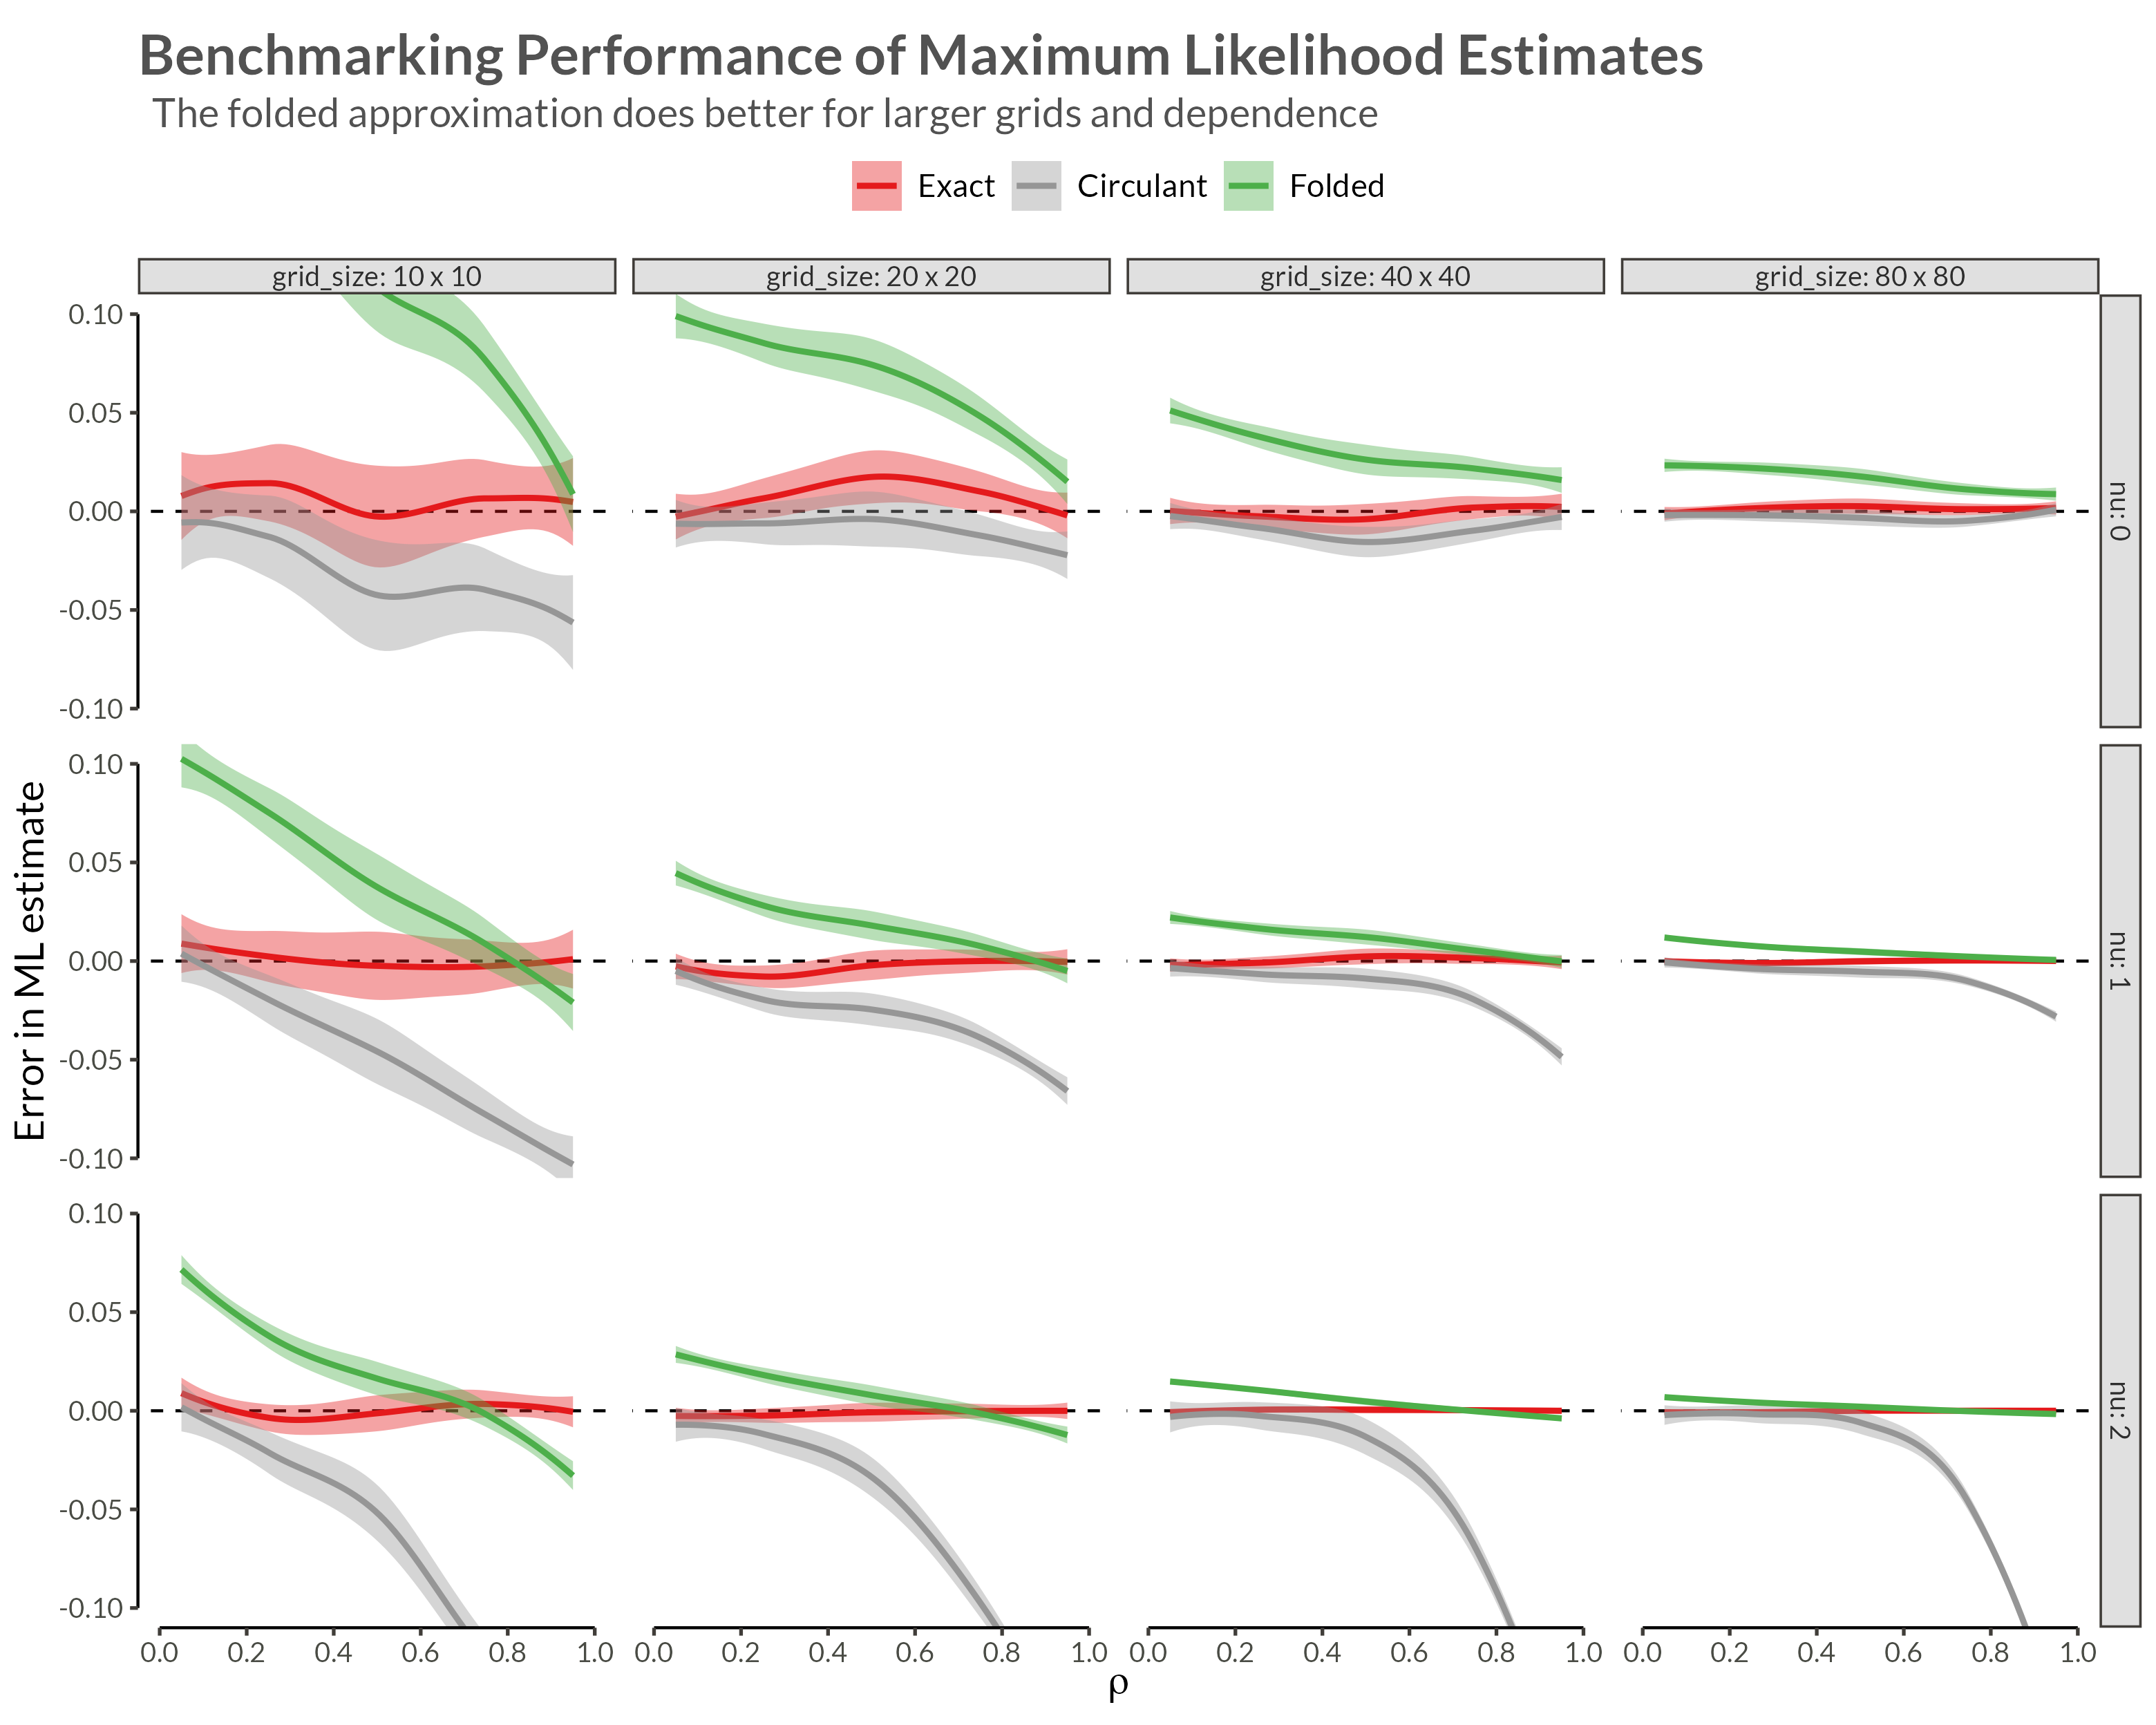
\includegraphics{images/bench_ml_bias.png}
\end{column}

\begin{column}{0.35\textwidth}

\begingroup
\fontsize{12.0pt}{14.4pt}\selectfont
\begin{longtable*}{llll}
\toprule
 &  & \multicolumn{2}{c}{Folded} \\ 
\cmidrule(lr){3-4}
Grid Size & Exact & Time & Speed-Up \\ 
\midrule\addlinespace[2.5pt]
10 x 10 & 6.86ms & 2.42ms & 2.84x \\ 
20 x 20 & 15.42ms & 7.64ms & 2.02x \\ 
30 x 30 & 35.02ms & 12.13ms & 2.89x \\ 
40 x 40 & 75.03ms & 19.43ms & 3.86x \\ 
50 x 50 & 150.24ms & 28.68ms & 5.24x \\ 
60 x 60 & 284.12ms & 40.26ms & 7.06x \\ 
70 x 70 & 485.3ms & 54.8ms & 8.86x \\ 
80 x 80 & 754.37ms & 74.66ms & 10.1x \\ 
\bottomrule
\end{longtable*}
\endgroup
\end{column}
\end{columns}
\end{frame}

\begin{frame}{Approximating the Correlation Matrix}
\phantomsection\label{approximating-the-correlation-matrix}
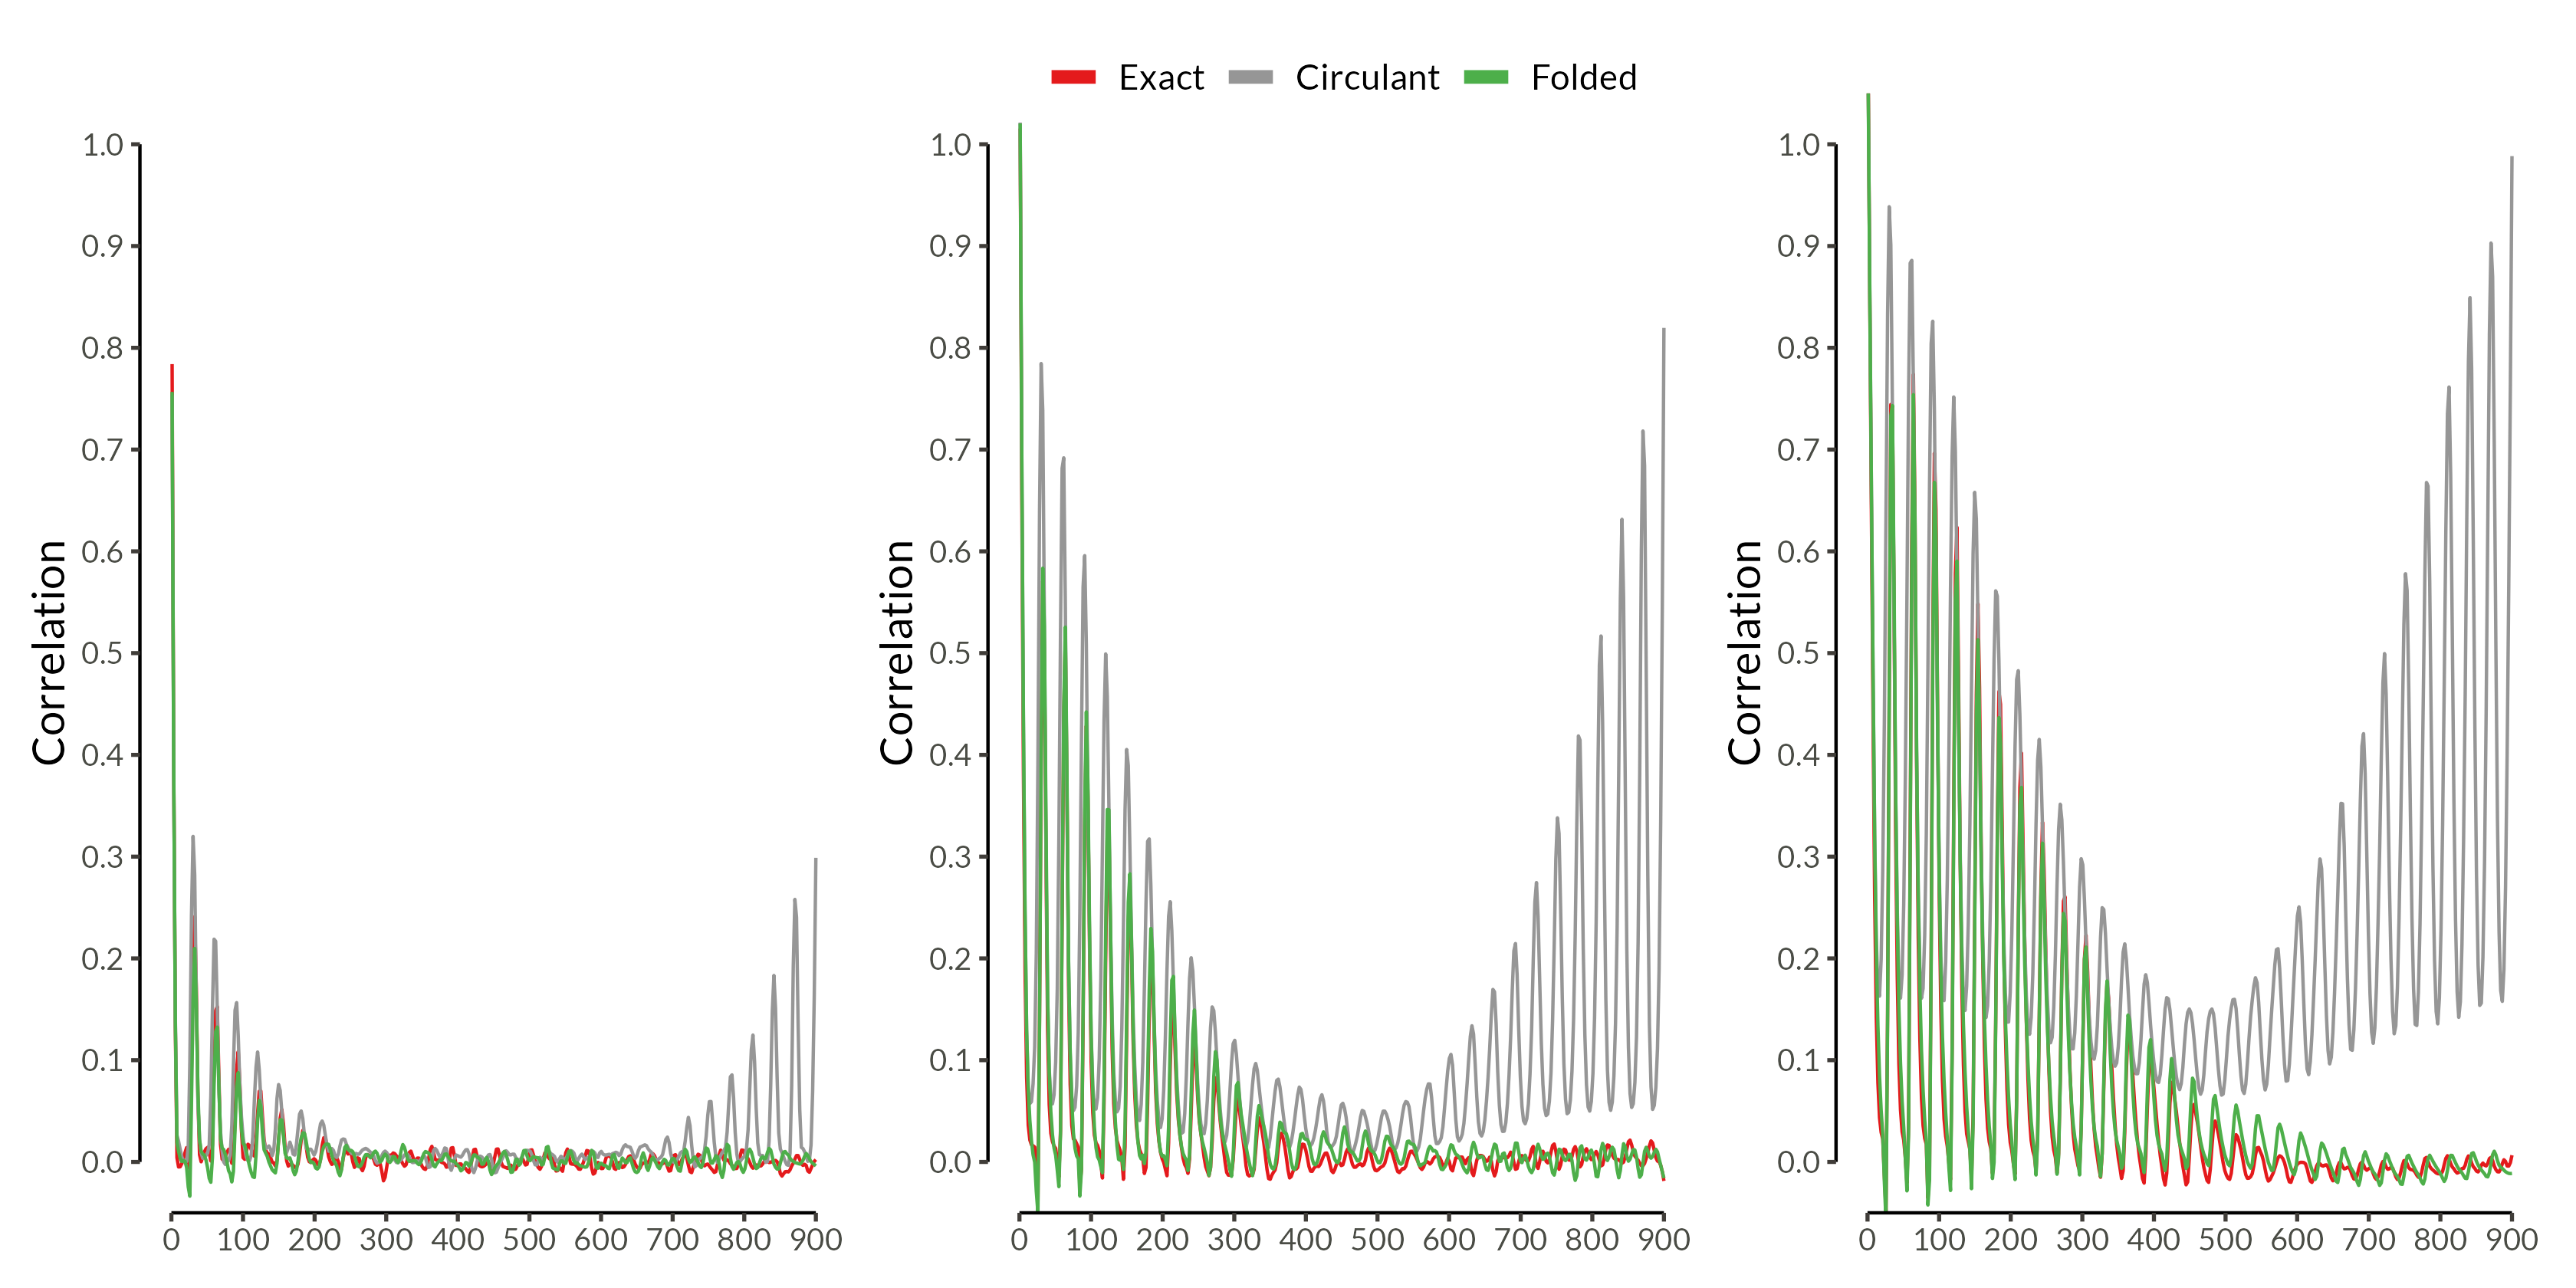
\includegraphics{images/cors.png}
\end{frame}

\begin{frame}[fragile]{Data Generation}
\phantomsection\label{data-generation}
\begin{columns}[T]
\begin{Shaded}
\begin{Highlighting}[]
\NormalTok{tictoc}\SpecialCharTok{::}\FunctionTok{tic}\NormalTok{()}
\NormalTok{X }\OtherTok{\textless{}{-}} \FunctionTok{rmatern\_copula\_folded\_full}\NormalTok{(}\AttributeTok{n =} \DecValTok{100}\NormalTok{, }\AttributeTok{dim1 =} \DecValTok{200}\NormalTok{, }\AttributeTok{dim2 =} \DecValTok{90}\NormalTok{, }\AttributeTok{rho1 =} \FloatTok{0.8}\NormalTok{, }\AttributeTok{rho2 =} \FloatTok{0.9}\NormalTok{, }\AttributeTok{nu =} \DecValTok{2}\NormalTok{)}
\NormalTok{tictoc}\SpecialCharTok{::}\FunctionTok{toc}\NormalTok{()}
\end{Highlighting}
\end{Shaded}

\begin{verbatim}
0.262 sec elapsed
\end{verbatim}

\begin{column}{50%;text-align:center\textwidth}
\begin{Shaded}
\begin{Highlighting}[]
\FunctionTok{plot\_matern}\NormalTok{(X[, }\DecValTok{1}\NormalTok{], }\DecValTok{200}\NormalTok{, }\DecValTok{90}\NormalTok{)}
\end{Highlighting}
\end{Shaded}

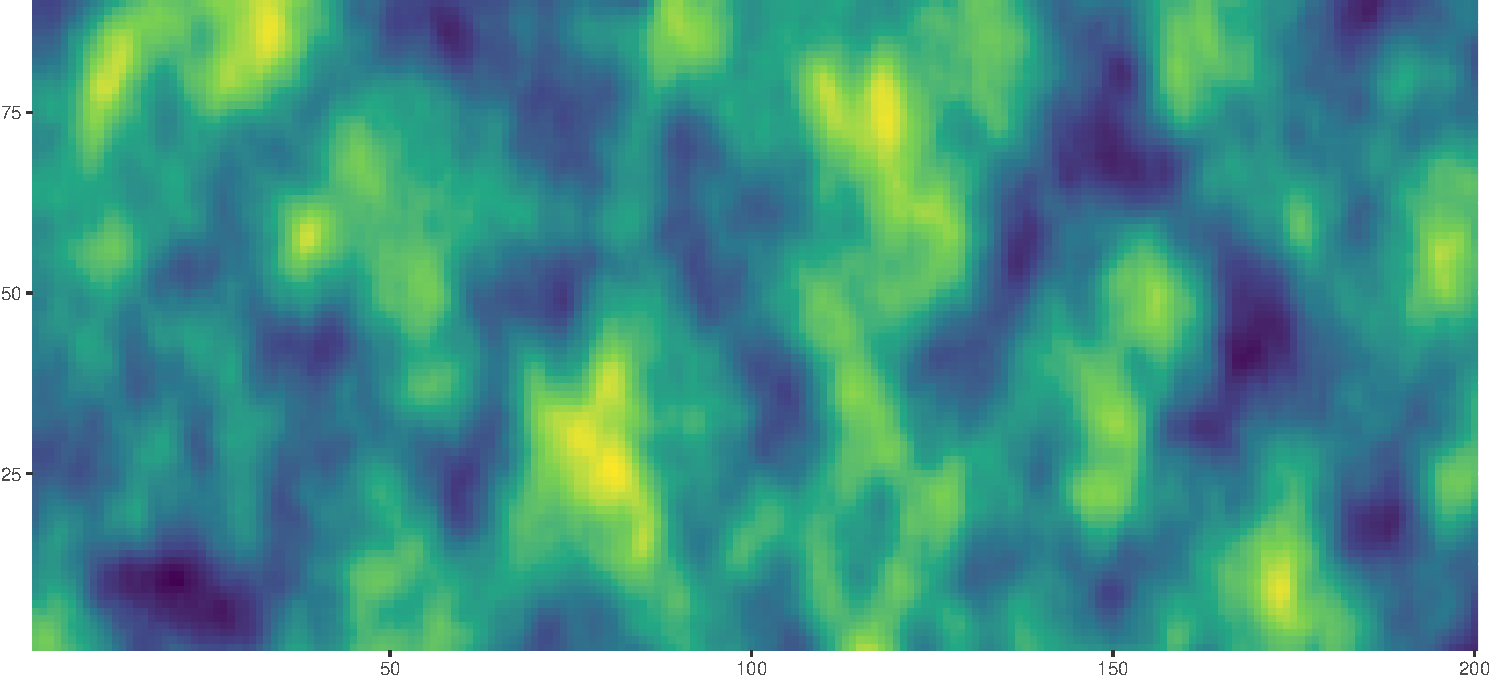
\includegraphics[width=0.8\textwidth,height=\textheight]{index_files/figure-beamer/unnamed-chunk-7-1.pdf}

\begin{Shaded}
\begin{Highlighting}[]
\FunctionTok{plot\_matern}\NormalTok{(X[, }\DecValTok{2}\NormalTok{], }\DecValTok{200}\NormalTok{, }\DecValTok{90}\NormalTok{)}
\end{Highlighting}
\end{Shaded}

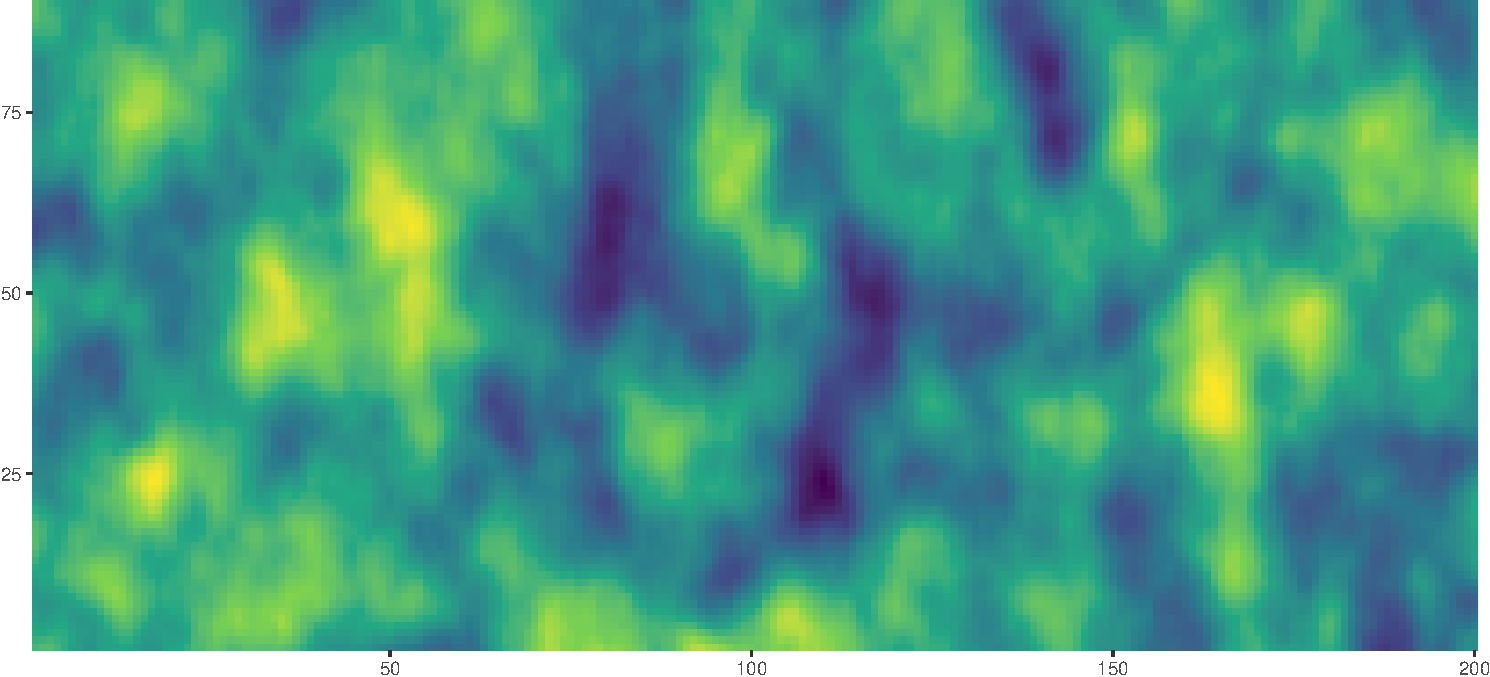
\includegraphics[width=0.8\textwidth,height=\textheight]{index_files/figure-beamer/unnamed-chunk-8-1.pdf}
\end{column}

\begin{column}{0.5\textwidth}
\begin{Shaded}
\begin{Highlighting}[]
\FunctionTok{apply}\NormalTok{(X, }\DecValTok{1}\NormalTok{, var) }\SpecialCharTok{|\textgreater{}} \FunctionTok{hist}\NormalTok{()}
\end{Highlighting}
\end{Shaded}

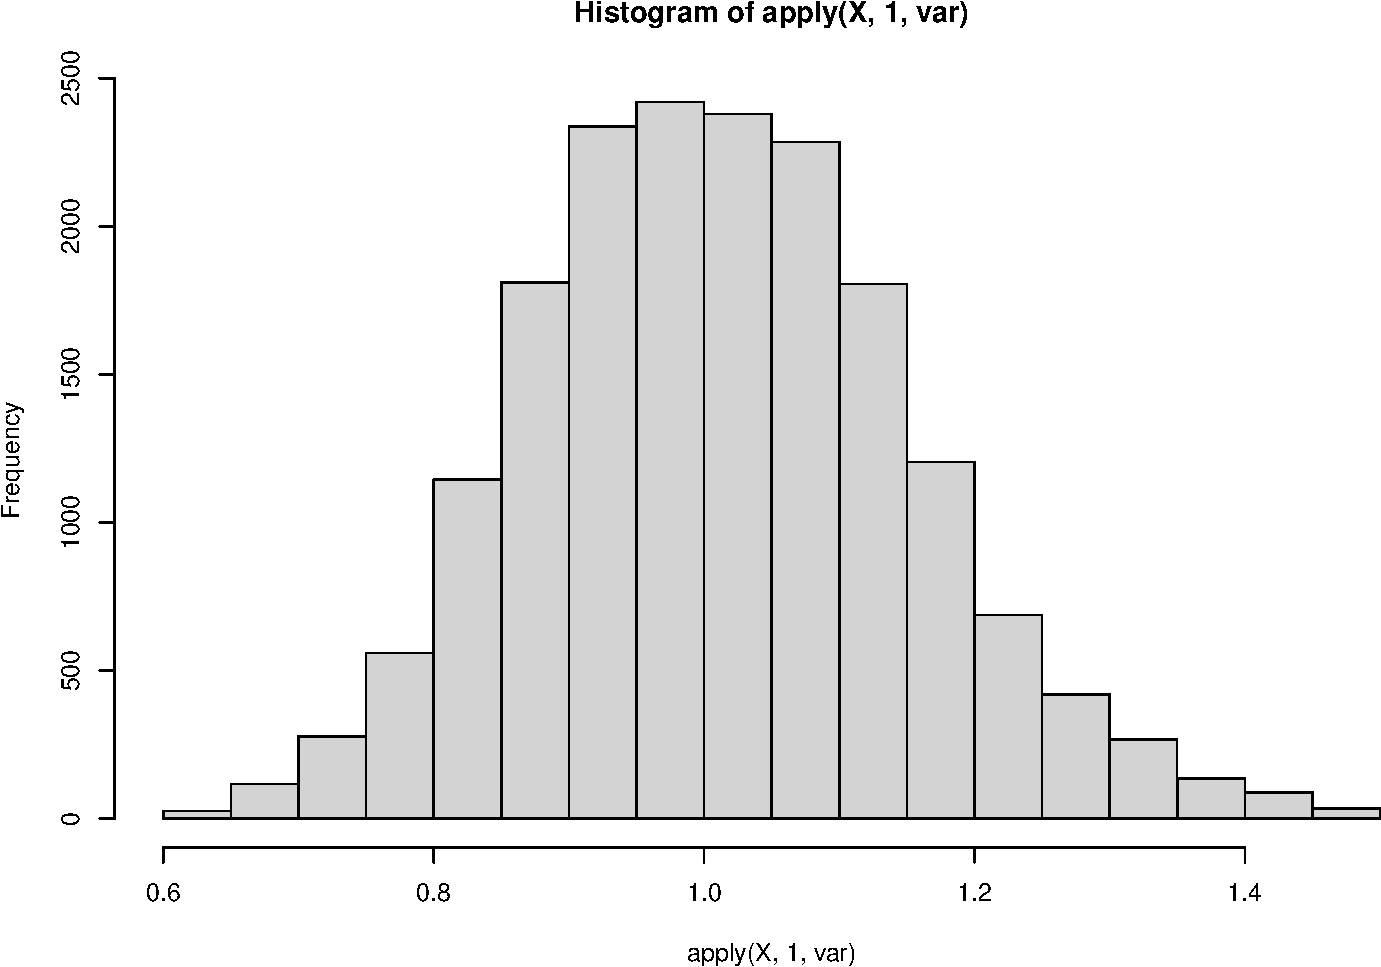
\includegraphics[width=0.8\textwidth,height=\textheight]{index_files/figure-beamer/unnamed-chunk-9-1.pdf}

\begin{Shaded}
\begin{Highlighting}[]
\FunctionTok{apply}\NormalTok{(X, }\DecValTok{1}\NormalTok{, mean) }\SpecialCharTok{|\textgreater{}} \FunctionTok{hist}\NormalTok{()}
\end{Highlighting}
\end{Shaded}

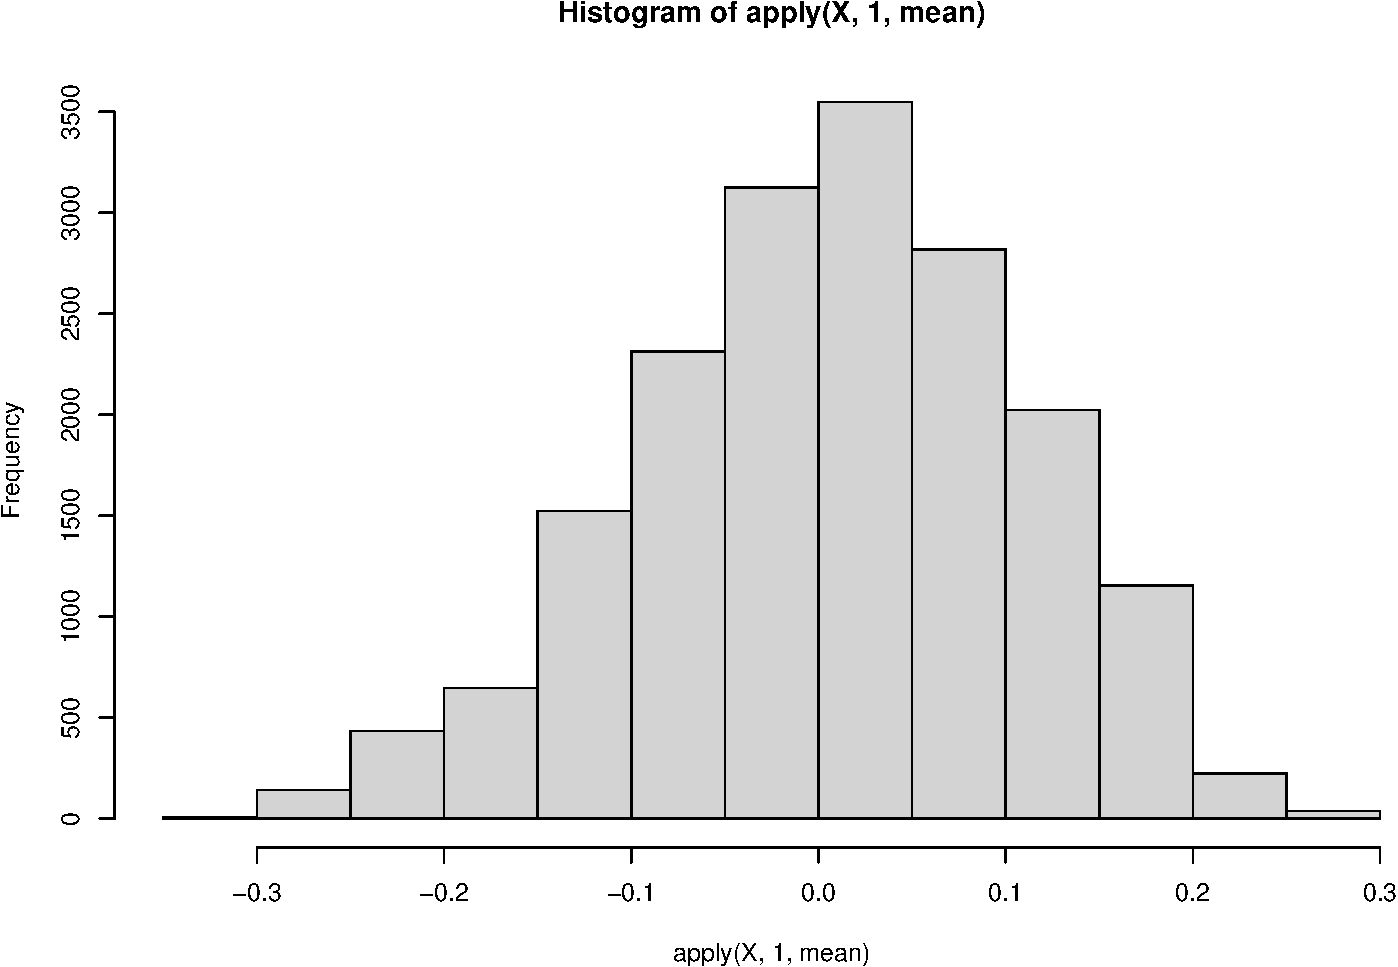
\includegraphics[width=0.8\textwidth,height=\textheight]{index_files/figure-beamer/unnamed-chunk-10-1.pdf}
\end{column}
\end{columns}
\end{frame}

\begin{frame}{Conclusion and Future Work}
\phantomsection\label{conclusion-and-future-work}
\begin{columns}[T]
\begin{column}{0.5\textwidth}
\begin{block}{Key Results}
\phantomsection\label{key-results}
\begin{itemize}
\tightlist
\item
  Developed Matérn-like Gaussian copula for large spatial fields
\item
  Folded circulant approximation to the density
\item
  Achieved fast density computations
\item
  Viable for MCMC samplers
\end{itemize}
\end{block}
\end{column}

\begin{column}{0.5\textwidth}
\begin{block}{Future Work}
\phantomsection\label{future-work}
\begin{itemize}
\tightlist
\item
  Investigate similar t-copulas
\item
  Perform simulation studies
\item
  Apply to other environmental and climate datasets
\end{itemize}
\end{block}
\end{column}
\end{columns}
\end{frame}




\end{document}
